\documentclass[11pt,oneside,openany]{book}
\usepackage[T1]{fontenc}
\usepackage[utf8]{inputenc}
\usepackage{lmodern}
\usepackage{amsmath,amssymb,amsthm,mathtools}
\usepackage{geometry,booktabs,longtable,array,enumitem,microtype,xcolor}
\usepackage[colorlinks=true,linkcolor=black,citecolor=black,urlcolor=blue!50!black,breaklinks=true]{hyperref}
\usepackage{fancyhdr}
\usepackage{titlesec}
\usepackage{tocloft}
\setlength{\cftbeforechapskip}{3pt}\setlength{\cftbeforesecskip}{0pt}
\titleclass{\chapter}{straight}
\titleformat{\chapter}[hang]{\normalfont\LARGE\bfseries\raggedright}{\chaptertitlename\ \thechapter}{0.6em}{}
\titlespacing*{\chapter}{0pt}{26pt}{14pt}

\usepackage{graphicx}
\usepackage{tikz}
\usetikzlibrary{arrows.meta,positioning,calc,decorations.pathreplacing}
\usepackage[font=small,labelfont=bf]{caption}
\geometry{a4paper,margin=28mm,headheight=14pt}
\setlength{\parindent}{0pt}
\setlength{\parskip}{5pt}
\setcounter{tocdepth}{2}
\pagestyle{fancy}
\fancyhf{}
\fancyhead[L]{\footnotesize Mathematical Foundations of the UNNS Substrate}
\fancyhead[R]{\footnotesize Volume I}
\fancyfoot[C]{\thepage}
\newtheorem{theorem}{Theorem}[chapter]
\newtheorem{proposition}[theorem]{Proposition}
\newtheorem{lemma}[theorem]{Lemma}
\newtheorem{corollary}[theorem]{Corollary}
\theoremstyle{definition}
\newtheorem{definition}[theorem]{Definition}
\newtheorem{example}[theorem]{Example}
\theoremstyle{remark}
\newtheorem{remark}[theorem]{Remark}
\newcommand{\Q}{\mathbb{Q}}
\newcommand{\N}{\mathbb{N}}
\newcommand{\Z}{\mathbb{Z}}
\newcommand{\Fx}{\mathcal{F}}
\newcommand{\Dx}{\mathcal{D}}
\newcommand{\lcmop}{\operatorname{lcm}}
\newcommand{\gcdop}{\operatorname{gcd}}
\newcommand{\ord}{\operatorname{ord}}
\newcommand{\Pred}{\operatorname{Pred}}
\newcommand{\Desc}{\operatorname{Desc}}
\newcommand{\Min}{\operatorname{Min}}
\newcommand{\scope}[1]{\textsf{\small Scope #1.}\ }
\newcommand{\record}[1]{\textup{\textsc{Source record: #1.}}\ }
\newcommand{\srcpath}[1]{\href{https://github.com/ukbbi/UNNS/blob/bb8b12d753c600c597feb00df17fe139c7cc65fa/projects/UNNS_MATH_FOUNDATIONS/sources/#1}{\nolinkurl{sources/#1}}}
\newcommand{\src}[2]{\href{https://github.com/ukbbi/UNNS/blob/bb8b12d753c600c597feb00df17fe139c7cc65fa/projects/UNNS_MATH_FOUNDATIONS/sources/#1}{#2}}
\newcommand{\Gen}{\mathcal{G}}
\tikzset{box/.style={draw,rounded corners=2pt,align=center,inner sep=4pt,font=\small},
 pt/.style={circle,fill=black,inner sep=1.4pt},lab/.style={font=\footnotesize}}
\newcommand{\Rh}{\mathcal{R}}
\newcommand{\join}{J_{\mathrm{join}}}
\newcommand{\jref}{J_{\mathrm{ref}}}
\newcommand{\Del}{\Delta}
\newcommand{\nohist}{H_{\mathrm{hist}}}
\begin{document}
\frontmatter
\begin{titlepage}
\centering
\vspace*{30mm}
{\Large THE MATHEMATICAL FOUNDATIONS\par}
\vspace{4mm}
{\Large OF THE UNNS SUBSTRATE\par}
\vspace{17mm}
{\Huge\bfseries Volume I\par}
\vspace{5mm}
{\LARGE Generative Arithmetic and\par Structural Reachability\par}
\vspace{20mm}
{\large Generative Structures, Reachability, Interaction,\par and Arithmetic Dynamics\par}
\vfill
{\large Working manuscript\par}
{\large 23 October 2026\par}
\vspace{6mm}
{\normalsize Source baseline: GitHub reference collection\par commit \texttt{bb8b12d753c600c597feb00df17fe139c7cc65fa}\par}
\end{titlepage}
\chapter*{Abstract}
\addcontentsline{toc}{chapter}{Abstract}
In the UNNS Substrate, numerical equality need not imply equality of generative structure. Distinct nested occurrences may realize the same value while retaining different routes, common futures, and structural relationships. This volume develops a mathematical theory of that generative multiplicity and establishes its consequences for arithmetic structure, reachability, rigidity, and interaction.

We derive an exact characterization of rational occurrence fibres, determine the arithmetic lattices governing common route continuations, and establish an integral coherence invariant for collective rendezvous. The resulting weighted fibre geometry admits a classification of three-route structures, including infinite families of rigid configurations.

We then investigate how generative structure changes under distinct continuation rules. Factor amplification and refinement yield different order-theoretic operations on anchor routes. Integer self-substitution produces an acyclic arithmetic graph whose edges are precisely the cover relations of its reachability order. This graph is non-graded, possesses neither universal joins nor universal meets, and distinguishes numerical endpoints, incoming routes, and complete generative histories.

Finally, we establish a structural nonselection principle and prove an incompatibility theorem: on the full occurrence-pair domain, common-future admissibility, stationarity, and weak label-blindness cannot simultaneously govern a value-valued interaction. This identifies a precise mathematical boundary between the structure generated by arithmetic rules and the additional specifications required for collective interaction.

Together, these results provide a unified foundation for studying generation, structural distinction, admissibility, and interaction within UNNS. Volume II extends this foundation through an explicitly defined collective dynamical system, establishing, as theorems about that map, unbounded fibre growth, eventual exact scaling, single-prime rigidity, arithmetic survivor selection, and effective bounds on transient evolution.

\chapter*{Introduction: the Substrate and the subject of this volume}
\addcontentsline{toc}{chapter}{Introduction: the Substrate and the subject of this volume}
\textbf{The Substrate.} UNNS treats recursion, rather than quantity, as the primitive. Its basic object is the nested number sequence: for fixed \(N\), the occurrences \((M,N)\), \(M=1,2,\dots\), carry the values \(M(N+1)^2/N\), an arithmetic progression with increment \((N+1)^2/N\). This volume develops the arithmetic and generative foundations of the Substrate: the structure carried by this rule and by the generative systems built directly on it. Later operators and field dynamics rest on these foundations and are outside this volume. Every statement here concerns the occurrences, fibres, routes and nests of the Substrate.

\textbf{The central object: the fibre.} Different occurrences can carry the same value. The set of occurrences carrying a value \(x\) is its \emph{fibre}, and its size \(R(x)\) measures how many distinct routes the Substrate offers to reach \(x\). Chapter~\ref{ch:objects} shows that this set is finite and describes it exactly. Chapters~\ref{ch:rendezvous} and \ref{ch:rigidity} study how routes through one value meet again in the future and how distinguishable they are from each other. These are the questions one must settle before asking how routes \emph{interact}.

\textbf{Forced versus chosen.} The guiding distinction of the volume is between what the nest rule determines and what is added by a choice. Each result is therefore labelled with its \emph{scope}: \textsf{A0}, elementary occurrence arithmetic, which depends on the nest rule alone; \textsf{A1}, the anchor-route and amplification systems of SELECT-I, which add an explicit generative step; \textsf{A2}, the integer self-substitution graph of SELECT-II, which adds the rule that an integer output may serve as the next input; and \textsf{X}, results about axioms any interaction law might satisfy. No theorem of this volume asserts that \textsf{A0} forces a unique \textsf{A1}, \textsf{A2}, or interaction law, and the final chapter proves why: the constraints that look natural are either too weak to select one operation or jointly incompatible.

\textbf{Reading the volume.} Chapters~\ref{ch:objects}--\ref{ch:rigidity} are arithmetic (\textsf{A0}). Chapter~\ref{ch:selection} treats the two readings of the nest rule built from anchor routes (\textsf{A1}); Chapters~\ref{ch:graph} and \ref{ch:histories} treat the integer graph and its histories (\textsf{A2}); Chapter~\ref{ch:nonselection} treats interaction axioms (\textsf{X}) and states the bridge to Volume II, which studies one explicitly adopted collective rule \(C(x)=x+L(x)^2/G(x)\). Each theorem carries a source-record tag (for example F.T1 or S2.4). These refer to the preserved FIELD-I, SELECT-I and SELECT-II records, pinned to the GitHub reference commit \texttt{bb8b12d}, and to the editorial registry of 128 records; the crosswalk in Appendix~\ref{app:crosswalk} lists all 60 records assigned to this volume together with their registered status. Statements that rest on finite computation are marked as such and are never presented as theorems.

\textbf{The wider architecture.} The Substrate programme proceeds from a recursive substrate through nested generation, routes, boundaries and admissibility to persistence and transition, and finally to observable structure. Volume I supplies the mathematics of generation, routes, reachability and the specification of interaction; Volume II develops persistence, arithmetic selection and long-term evolution under one explicitly specified map. Neither volume by itself proves every claim associated with the broader architecture; each establishes what its theorems state.

\begin{figure}[t]
\centering
\resizebox{0.97\linewidth}{!}{\begin{tikzpicture}[>=Stealth,font=\scriptsize]
\tikzset{st/.style={draw,rounded corners=2pt,align=center,inner sep=3pt,text width=1.75cm,minimum height=0.95cm}}
\node[st] (n1) at (0,0) {Recursive\\ substrate};
\node[st] (n2) at (2.15,0) {Nested\\ generation};
\node[st] (n3) at (4.3,0) {Routes};
\node[st,fill=black!5] (n4) at (6.45,0) {Boundaries};
\node[st,fill=black!5] (n5) at (8.6,0) {Admissibility};
\node[st] (n6) at (10.75,0) {Persistence and transition};
\node[st,fill=black!5] (n7) at (12.9,0) {Observable structure};
\foreach \a/\b in {n1/n2,n2/n3,n3/n4,n4/n5,n5/n6,n6/n7} \draw[->] (\a) -- (\b);
\draw[decorate,decoration={brace,mirror,amplitude=4pt}] (-0.8,-0.75) -- node[below=5pt,align=center]{Volume I: generation, routes,\\ reachability, specification of interaction} (5.1,-0.75);
\draw[decorate,decoration={brace,mirror,amplitude=4pt}] (9.95,-0.75) -- node[below=5pt,align=center]{Volume II: persistence, arithmetic\\ selection, evolution under a specified map} (13.7,-0.75);
\end{tikzpicture}}
\caption{The broader Substrate architecture and the part developed in the two volumes. Shaded stages are not developed in either volume.}
\end{figure}

\begin{figure}[t]
\centering
\begin{tikzpicture}[>=Stealth]
\node[box] (a0) at (0,0) {\textsf{A0}\\ nest-rule arithmetic\\ Ch.~\ref{ch:objects}--\ref{ch:rigidity}};
\node[box] (a1) at (6.2,1.7) {\textsf{A1}\\ anchor routes, amplification,\\ refinement (Ch.~\ref{ch:selection})};
\node[box] (x) at (6.2,0) {\textsf{X}\\ axioms for interaction laws\\ (Ch.~\ref{ch:nonselection})};
\node[box] (a2) at (6.2,-1.7) {\textsf{A2}\\ integer self-substitution graph\\ (Ch.~\ref{ch:graph}--\ref{ch:histories})};
\node[box,fill=black!6] (v2) at (11.6,0) {Volume II\\ collective map $C$\\ (explicitly adopted)};
\draw[->] (a0) -- node[lab,above,sloped]{adds a step} (a1);
\draw[->] (a0) -- node[lab,above]{no new rule} (x);
\draw[->] (a0) -- node[lab,below,sloped]{adds a rule} (a2);
\draw[->,thick] (x) -- node[lab,above]{choice of $C$} (v2);
\draw[->,dashed,gray] (a1.east) to[out=0,in=100] node[lab,above right,pos=.7,text=black]{no implication} (v2.north);
\draw[->,dashed,gray] (a2.east) to[out=0,in=-100] (v2.south);
\end{tikzpicture}
\caption{Architecture of Volume I. Scope \textsf{A0} depends on the nest rule alone; \textsf{A1} and \textsf{A2} are two different explicit generative readings of it; \textsf{X} studies which axioms an interaction law can satisfy. Dashed arrows mark what is \emph{not} implied: neither \textsf{A1} nor \textsf{A2} forces the collective map $C$ of Volume~II.}
\end{figure}
\tableofcontents
\mainmatter

\chapter{Formal Objects and Generative Arithmetic}
\label{ch:objects}
\section{Occurrences, values and fibres}
We begin with a positive-rational occurrence rule, considered here simply as a formally specified arithmetic construction. For \(N,M\in\N_{>0}\), put
\begin{equation}\label{eq:base}
 S_N(M)=\frac{M(N+1)^2}{N}.
\end{equation}
Nothing in this definition prescribes substitution, pairwise interaction, or a future orbit. At fixed \(N\), the sequence of occurrences \((M,N)\) is an arithmetic progression in value, with increment \((N+1)^2/N\). Distinguish an \emph{occurrence} \((M,N)\) from its numerical value \(x=S_N(M)\): one value may arise from different occurrences.

\begin{definition}[Rational fibre and square-divisor index]\label{def:fibre}
For \(x\in\Q_{>0}\), its occurrence fibre is
\[
 \Fx(x)=\{(M,N)\in\N_{>0}^2:S_N(M)=x\},\qquad R(x)=|\Fx(x)|.
\]
For reduced \(x=a/b\), where \(a,b\in\N_{>0}\) and \(\gcdop(a,b)=1\), define
\[
 \Dx(x)=\{d\in\N:d\ge2,\ d^2\mid a,\ d\equiv 1\pmod b\}.
\]
The integer \(d=N+1\) is the \emph{index} of an occurrence. The symbol \(R(x)\) always denotes fibre multiplicity, not an eventual-transient bound.
\end{definition}

\begin{theorem}[Rational-fibre characterization]\label{thm:fibre}
\scope{A0}\record{F.T1} For reduced \(x=a/b>0\), the map \((M,N)\mapsto d=N+1\) is a bijection \(\Fx(x)\to\Dx(x)\), with inverse
\begin{equation}\label{eq:occ-inverse}
 N=d-1,\qquad M=\frac{a}{d^2}\frac{d-1}{b}.
\end{equation}
In particular, \(R(x)=|\Dx(x)|\) is finite.
\end{theorem}
\begin{proof}
The equality \(a/b=Md^2/(d-1)\) gives
\(bMd^2=a(d-1)\). Because \(\gcdop(d^2,d-1)=1\), we have \(d^2\mid a\), so write \(a=kd^2\). Then \(bM=k(d-1)\). Since \(\gcdop(a,b)=1\) and \(d^2\mid a\), also \(\gcdop(k,b)=1\), whence \(b\mid(d-1)\). Conversely, a \(d\) satisfying the divisibility and congruence conditions makes \(M=k(d-1)/b\) a positive integer, and substitution in \eqref{eq:base} gives \(a/b\). Uniqueness follows from \(d=N+1\).
\end{proof}

\begin{corollary}[Multiplicity for integer values]\label{cor:mult}
\scope{A0} For every \(m\in\N_{>0}\),
\begin{equation}\label{eq:mult}
 R(m)=\prod_{p\mid m}\left(\left\lfloor\frac{\nu_p(m)}2\right\rfloor+1\right)-1.
\end{equation}
In particular, \(R(m)=0\) if and only if \(m\) is squarefree.
\end{corollary}
\begin{proof}
For denominator one, \(\Dx(m)\) consists exactly of the square roots of nontrivial square divisors of \(m\). The exponent of \(p\) in such a root ranges from zero to \(\lfloor\nu_p(m)/2\rfloor\), independently of the other primes. Exclude the all-zero choice \(d=1\).
\end{proof}

\begin{example}[Anatomy of a fibre: \(x=72\)]\label{ex:anatomy}
Here \(72=2^3\cdot3^2\), so \(\Dx(72)=\{2,3,6\}\) and \(R(72)=3\). Equation~\eqref{eq:occ-inverse} gives the three occurrences, and each lies on its own nest with its own step:
\[
\begin{array}{c|c|c|c|c}
d & N=d-1 & M=\tfrac{72}{d^2}(d-1) & \text{anchor route }(k,d) & \text{step }d^2/(d-1)\\\hline
2&1&18&(18,2)&4\\
3&2&16&(8,3)&9/2\\
6&5&10&(2,6)&36/5
\end{array}
\]
Three different nests, with three different increments, pass through the same value. Figure~\ref{fig:routes72} shows how their later values interlace. The three routes agree again exactly at \(72,108,144,180,\dots\), in steps of \(L^2/G=36/\gcdop(1,2,5)=36\); this is the collective step of Theorem~\ref{thm:coll}. Note also that the numbers \(M=18,16,10\) are the predecessors of \(72\) in the graph of Chapter~\ref{ch:graph}; this is the dictionary of Theorem~\ref{thm:pred}.
\end{example}
\begin{figure}[t]
\centering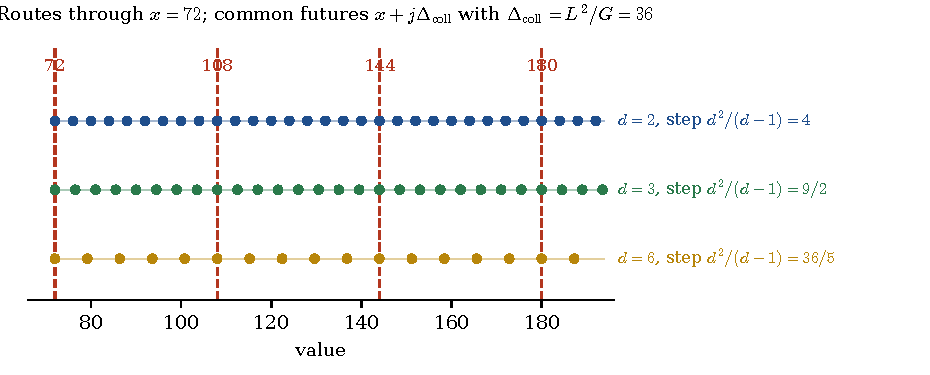
\includegraphics[width=\linewidth]{figs/fig_routes72.pdf}
\caption{The three routes through \(x=72\) (one row each, dots mark their values) and the common futures (dashed). Between consecutive common futures the three nests take $9$, $8$ and $5$ route steps (that is, $8$, $7$ and $4$ strictly intermediate values), and these never coincide before the collective step.}\label{fig:routes72}
\end{figure}
\begin{figure}[t]
\centering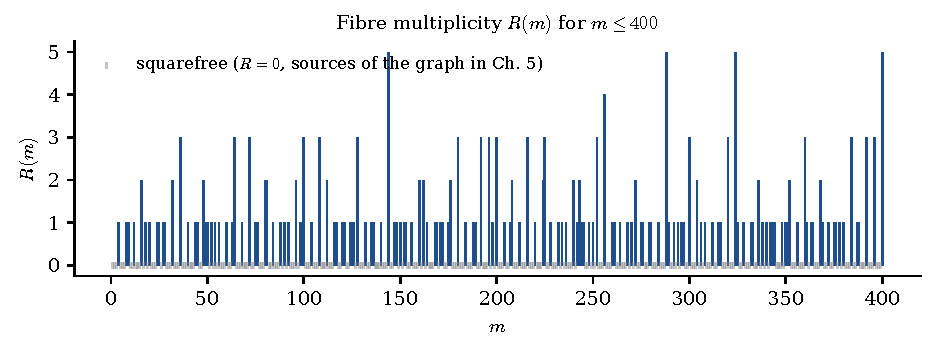
\includegraphics[width=\linewidth]{figs/fig_Rm.pdf}
\caption{The fibre multiplicity \(R(m)\) for \(m\le400\), from Corollary~\ref{cor:mult}. The zeros are the squarefree integers; larger values occur where a high square part makes many index choices available.}\label{fig:Rm}
\end{figure}

\begin{proposition}[Reparametrization and integer sub-fibres]\label{prop:reparam}
\scope{A0}\record{F.T1p, F.T1pp} Suppose \(M=kg\), \(N=bg\), with \(\gcdop(k,b)=1\). Then \(S_N(M)=k(bg+1)^2/b\) in lowest terms, and \(b=N/\gcdop(M,N)\). Furthermore the map \((M,N)\mapsto(bM,N)\) embeds \(\Fx(a/b)\) in \(\Fx(a)\), with image precisely the occurrences for \(a\) whose index satisfies \(b\mid N\). Thus \(R(a/b)\le R(a)\).
\end{proposition}
\begin{proof}
Substitution yields the stated fraction. Since \(bg+1\equiv1\pmod b\), its numerator is coprime to \(b\). To verify the second statement, multiply \(S_N(M)=a/b\) by \(b\), obtaining \(S_N(bM)=a\). Conversely, whenever \(b\mid N\), Theorem~\ref{thm:fibre} implies the corresponding numerator \(M\) for \(a\) is divisible by \(b\), giving the inverse construction.
\end{proof}

\section{Realisability and the square-root part}
\begin{theorem}[Arithmetic realisability]\label{thm:real}
\scope{A0}\record{F.T3} A reduced noninteger \(a/b>0\), \(b\ge2\), has a nonempty fibre if and only if its numerator possesses a square divisor \(d^2\) with \(d\ge2\), \(d\equiv1\pmod b\). Necessarily \(a\ge(b+1)^2\), and equality is attainable.
\end{theorem}
\begin{proof}
The equivalence is Theorem~\ref{thm:fibre}. Since the smallest integer \(d\ge2\) with \(d\equiv1\pmod b\) is \(d=b+1\), the lower bound follows from \(d^2\mid a\). Taking \(a=(b+1)^2\) gives the occurrence \((M,N)=(1,b)\) and gives a reduced fraction since \(\gcdop((b+1)^2,b)=1\).
\end{proof}

\begin{theorem}[Square-root reduction]\label{thm:sqrtpart}
\scope{A0}\record{F.T22} Write the positive integer numerator uniquely as \(a=s^2t\), with \(t\) squarefree and \(s\) the maximal square-root part. Then
\begin{equation}\label{eq:root}
 \Dx(a/b)=\{d\ge2:d\mid s,\ d\equiv1\pmod b\}.
\end{equation}
Consequently the pattern of indices of the fibre depends only on \((s,b)\), not on the squarefree factor \(t\). If \(q\) is squarefree and \(\gcdop(q,ab)=1\), then \(\Dx(qa/b)=\Dx(a/b)\).
\end{theorem}
\begin{proof}
For each prime \(p\), the inequality \(2\nu_p(d)\le\nu_p(a)\) is equivalent to \(\nu_p(d)\le\lfloor\nu_p(a)/2\rfloor=\nu_p(s)\). This is exactly \(d\mid s\). Multiplication of \(a\) by squarefree \(q\) coprime to \(a\) changes none of these floors; the denominator remains coprime to the numerator by the assumed coprimality.
\end{proof}

\begin{remark}[Primitive presentation of a fibre]
If \(\Dx(a/b)\ne\varnothing\) and \(\lambda=\lcmop\Dx(a/b)\), then \(\Dx(\lambda^2/b)=\Dx(a/b)\); this presents the same indices with the minimal divisor-lcm source. When speaking of a \emph{primitive pair} \((\lambda,b)\), we mean this index configuration, not an assertion that all numerical invariants of the two fibres are identical.
\end{remark}

\section{Refinement is distinct from continuation}
An integer-anchor route is \(r=(k,d)\) with \(k\ge1\), \(d\ge2\), and value \(v(r)=kd^2\). It corresponds to an integer occurrence with \(N=d-1\), \(M=k(d-1)\). Whenever \(q\ge1\) and \(q^2\mid k\), define a partial refinement
\[
 T_q(k,d)=\left(\frac{k}{q^2},dq\right).
\]
It preserves \(kd^2\) identically. For a reduced rational fibre \(a/b\) the analogous statement is Proposition~\ref{prop:refine} below. Neither the definition nor value preservation declares \(T_q\) to be a forward edge of a generative graph. That question is treated in Chapter~\ref{ch:selection}.

\begin{proposition}[Refinement and the rational fibre]\label{prop:refine}
\scope{A0}\record{F.T5} Let \(x=a/b\) be reduced, \(d\in\Dx(x)\), \(k=a/d^2\), and let \(q\ge2\) be an integer with \(q^2\mid k\). Then \(dq\in\Dx(x)\) if and only if \(q\equiv1\pmod b\).
\end{proposition}
\begin{proof}
Since \(q^2\mid k\), we have \((dq)^2=d^2q^2\mid d^2k=a\), so only the congruence condition remains. Because \(d\equiv1\pmod b\), \(dq\equiv q\pmod b\). Hence \(dq\equiv1\pmod b\) if and only if \(q\equiv1\pmod b\).
\end{proof}

\chapter{Common Futures and Rendezvous Lattices}\label{ch:rendezvous}
\section{The arithmetical future of a fixed occurrence}
Define the \emph{forward occurrence shift} \(F(M,N)=(M+1,N)\); this changes the value by
\[
 \sigma_N=\frac{(N+1)^2}{N}=\frac{d^2}{d-1}.
\]
For a route \(r=(M,N)\) through \(x\), the set of its values at nonnegative shift times is \(x+\sigma_N\Z_{\ge0}\). This operation moves \(M\) while leaving \(N\) fixed and must not be confused with the later SELECT-II substitution of a complete output as the new \(M\).

\begin{lemma}[Intersection of rational lattices]\label{lem:lcm}
\scope{A0}\record{F.L0} For reduced positive fractions \(u=p/q\), \(v=p'/q'\),
\[
 u\Z\cap v\Z=\frac{\lcmop(p,p')}{\gcdop(q,q')}\Z.
\]
\end{lemma}
\begin{proof}
For a nonzero rational \(z\) and a prime \(r\), write \(\nu_r\) for the \(r\)-adic valuation. Then \(z\in u\Z\) if and only if \(\nu_r(z)\ge\nu_r(u)\) for every prime \(r\). Hence \(u\Z\cap v\Z=w\Z\), where \(w>0\) satisfies \(\nu_r(w)=\max(\nu_r(u),\nu_r(v))\) for all \(r\). Fix \(r\). Because \(u,v\) are reduced, \(r\) divides at most one of \(p,q\) and at most one of \(p',q'\). If \(r\) divides neither \(q\) nor \(q'\), the maximum is \(\max(\nu_r(p),\nu_r(p'))=\nu_r(\lcmop(p,p'))\), and \(\nu_r(\gcdop(q,q'))=0\). If \(r\mid q\) but \(r\nmid q'\), then \(\nu_r(p)=0\) and the maximum is \(\nu_r(p')=\nu_r(\lcmop(p,p'))\), while \(\nu_r(\gcdop(q,q'))=0\); the case \(r\mid q'\), \(r\nmid q\) is symmetric. If \(r\) divides both denominators, then \(\nu_r(p)=\nu_r(p')=0\) and the maximum is \(-\min(\nu_r(q),\nu_r(q'))=-\nu_r(\gcdop(q,q'))\), while \(\nu_r(\lcmop(p,p'))=0\). In every case \(\nu_r(w)=\nu_r(\lcmop(p,p'))-\nu_r(\gcdop(q,q'))\), so \(w=\lcmop(p,p')/\gcdop(q,q')\).
\end{proof}

\begin{theorem}[Common-future lattice for a pair]\label{thm:pair}
\scope{A0}\record{F.T2, F.T6} Let \(r,s\in\Fx(x)\) be distinct, with indices \(d,d'\ge2\), hence \(N=d-1\), \(N'=d'-1\). Put
\[
 L_{rs}=\lcmop(d,d'),\quad g_{rs}=\gcdop(d-1,d'-1),\quad
 \Del_{rs}=\frac{L_{rs}^2}{g_{rs}}.
\]
Then their common future values are exactly
\begin{equation}\label{eq:common}
 \{x+j\Del_{rs}:j\in\Z_{\ge0}\}.
\end{equation}
\end{theorem}
\begin{proof}
Both routes pass through \(x\) and thereafter advance by steps \(d^2/(d-1)\), \(d'^2/(d'-1)\). Each is reduced because \(\gcdop(d^2,d-1)=1\). By Lemma~\ref{lem:lcm}, the intersection of their additive step lattices is generated by
\(\lcmop(d^2,d'^2)/\gcdop(d-1,d'-1)=L_{rs}^2/g_{rs}\). Intersecting the positive rays emanating from their shared value gives \eqref{eq:common}.
\end{proof}

\begin{theorem}[Integral pair index]\label{thm:pairindex}
\scope{A0}\record{F.T7} For reduced \(x=a/b\), define \(h_{rs}=x/\Del_{rs}\). Then
\[
 h_{rs}=\frac{a}{L_{rs}^2}\frac{g_{rs}}b\in\N_{>0},\qquad
 x< x+\Del_{rs}=x\left(1+\frac1{h_{rs}}\right)\le2x.
\]
\end{theorem}
\begin{proof}
Since \(d^2,d'^2\mid a\), we have \(L_{rs}^2\mid a\). Each occurrence has \(N\equiv0\pmod b\) by Theorem~\ref{thm:fibre}, so \(b\mid g_{rs}\). The index is therefore a positive integer. The inequality follows from \(h_{rs}\ge1\).
\end{proof}

\begin{example}[The first collective meeting is not a chosen interaction]
Let \(x=36\) and choose indices \(d=2\), \(d'=3\). Then \(L=6\), \(g_{rs}=1\), \(\Del_{rs}=36\), and the common futures are \(36,72,108,\ldots\). The existence of this arithmetic progression does not select a unique positive shift \(j\), a composition law on occurrences, or an interpretation as a physical meeting.
\end{example}

\section{Collective common futures}
For \(\Fx(x)\ne\varnothing\), let \(D=\Dx(x)\). Set \(L(x)=\lcmop D\) and \(G(x)=\gcdop\{d-1:d\in D\}\). As in the source, these quantities are defined for all nonempty fibres, including singleton fibres.
\begin{theorem}[Collective rendezvous and coherence]\label{thm:coll}
\scope{A0}\record{F.T8} The common future values of all routes in \(\Fx(x)\) form
\begin{equation}\label{eq:delta-coll}
 x+\Del_{\mathrm{coll}}(x)\Z_{\ge0},\qquad
 \Del_{\mathrm{coll}}(x)=\frac{L(x)^2}{G(x)}.
\end{equation}
For \(R(x)\ge2\), this step is the lattice-lcm of the pairwise \(\Del_{rs}\). Moreover
\[
 \gamma(x)=\frac{x}{\Del_{\mathrm{coll}}(x)}=\frac{G(x)x}{L(x)^2}
\]
is a positive integer, and for \(R(x)\ge2\), \(\gamma(x)=\gcdop\{h_{rs}:r\ne s\in\Fx(x)\}\).
\end{theorem}
\begin{proof}
Apply Lemma~\ref{lem:lcm} to the entire finite family of reduced route steps. Their numerator lcm is \(\lcmop_{d\in D}(d^2)=L^2\) and their denominator gcd is \(G\). For \(R\ge2\), taking lattice-lcms of pairwise steps gives the same numerator and denominator operations, hence coherence. Each \(d^2\mid a\), so \(L^2\mid a\), and \(b\mid(d-1)\) for all \(d\), so \(b\mid G\). Thus \(\gamma=(a/L^2)(G/b)\) is integral. Finally \(h_{rs}=x/\Del_{rs}\), while \(\Del_{\mathrm{coll}}\) is the least common multiple of all \(\Del_{rs}\) in the lattice sense. Therefore \(\gamma\mid h_{rs}\) for each pair. If \(c\) divides every \(h_{rs}\), then \(x/c\) is an integer multiple of every \(\Del_{rs}\), hence of \(\Del_{\mathrm{coll}}\); thus \(c\mid\gamma\). This establishes the gcd identity.
\end{proof}

\begin{corollary}[The pair-index spectrum is not a selection rule]\label{cor:pairspec}
\scope{A0}\record{F.T9} Every positive integer arises as a pair index. Indeed, for \(x=36h\), the indices \(d=2,3\) give \(\Del_{rs}=36\), hence \(h_{rs}=h\). Nevertheless neither \(h_{rs}\) nor \(\gamma(x)\) specifies which admissible common future is an interaction output.
\end{corollary}

\section{Rational index closures and their limits}
\begin{theorem}[Conditional joins and meets of fibre indices]\label{thm:join-fibre}
\scope{A0}\record{F.T16, correcting F.T4} If \(d,d'\in\Dx(a/b)\), then
\[
 \lcmop(d,d')\in\Dx(a/b)\iff\gcdop(d,d')\equiv1\pmod b,
\]
whereas
\[
 \gcdop(d,d')\in\Dx(a/b)\iff
 \gcdop(d,d')\ge2\text{ and }\gcdop(d,d')\equiv1\pmod b.
\]
For integer fibres \(b=1\), \(\Dx(m)\) is lcm-closed; it need not be a lattice on the declared domain \(d\ge2\). For rational \(b>1\), even its lcm may be inadmissible.
\end{theorem}
\begin{proof}
Since \(d^2,d'^2\mid a\), their lcm squared divides \(a\), and so does the square of their gcd. Write \(c=\gcdop(d,d')\), \(\ell=\lcmop(d,d')=dd'/c\). Because \(d,d'\equiv1\pmod b\), both are units modulo \(b\), hence \(\ell\equiv c^{-1}\pmod b\). Thus \(\ell\equiv1\) exactly when \(c\equiv1\). The gcd \(c\) must also satisfy the defining inequality \(c\ge2\). For \(b=1\) the congruence is automatic. The exceptional case \(c=1\) shows why the internal meet may be absent.
\end{proof}

\begin{example}[Failure of index-join closure]
For \(x=400/3\) the fibre index set is \(D=\{4,10\}\), but \(\lcmop(4,10)=20\not\equiv1\pmod3\). The arithmetic obstruction concerns this index structure, not the later self-iteration graph's reachability order.
\end{example}

\chapter{Fibre Rigidity and Three-Route Structures}\label{ch:rigidity}
\section{Weighted route geometry without a chosen interaction}
For a fibre with at least two indices define the pair weight and pair index by
\begin{equation}\label{eq:weight}
 w(d,e)=\frac{\gcdop(d-1,e-1)}{\lcmop(d,e)^2}
 =\frac1{\Del_{de}},\qquad
 h_{de}=xw(d,e).
\end{equation}
This quantity is determined by the arithmetic of common futures. It is not itself the metric or nonlinear excess associated with the proposed route join of the earlier relational-invariants program. It is also not a claim that a physical interaction exists between the indices.

\begin{definition}[Weighted fibre graph and rigidity]
On the finite vertex set \(\Dx(x)\), form the complete graph whose edge \(\{d,e\}\) carries weight \(w(d,e)\), equivalently the pair index \(h_{de}\). Call the fibre \emph{rigid} when this weighted graph admits no nontrivial vertex automorphism. For three indices, rigidity is equivalent to having three distinct edge weights.
\end{definition}
The last equivalence is specific to three vertices. If all three weights are distinct, every vertex is distinguished by its incident weights. If two weights agree, transposing their nonshared endpoints preserves the weighted triangle. For higher multiplicity, the corresponding graph-automorphism question must be considered on its own terms.

\begin{theorem}[Integer fibres of multiplicity three]\label{thm:int-three}
\scope{A0}\record{F.T20} If \(m\) is an integer with \(R(m)=3\), then, up to renaming primes, its fibre indices are precisely of one of the forms
\[
 \{p,q,pq\}\quad(p,q\text{ distinct primes}),\qquad
 \{p,p^2,p^3\}.
\]
Every such weighted three-route fibre is nonrigid.
\end{theorem}
\begin{proof}
By square-divisor closure, \(\Dx(m)\) is closed under positive divisors at least two and under lcm. If at least three distinct primes occur among its elements, the divisors \(p,q,r,pq\) already force four indices. For exactly two distinct primes, divisor and lcm closure and cardinality three force \(\{p,q,pq\}\). For one distinct prime, all indices are powers of that prime, and divisor closure plus cardinality three forces \(\{p,p^2,p^3\}\).

For the first form, the three pair lcms are all \(pq\); moreover
\(\gcdop(p-1,pq-1)=\gcdop(p-1,q-1)\), with the analogous identity for \(q\). The three edge weights therefore agree. In the second form, the weights for \(\{p,p^3\}\) and \(\{p^2,p^3\}\) coincide: both gcds of the respective indices minus one equal \(p-1\), and both lcms equal \(p^3\). Thus in either case the weighted triangle has a nontrivial automorphism.
\end{proof}

\section{Index closure lemmas and three-element shapes}
\begin{lemma}[Quotient and gcd closure]\label{lem:shape-closure}
\scope{A0}\record{F.T23} Put \(D=\{d\mid s:d\ge2,\ d\equiv1\pmod b\}\). Then:
\begin{enumerate}[label=(\alph*)]
\item If \(d\mid e\) with \(d,e\in D\), the quotient \(e/d\) is either one or an element of \(D\).
\item If \(d,e\in D\) and \(c=\gcdop(d,e)\equiv1\pmod b\), then \(\lcmop(d,e)\in D\), and \(c=1\) or \(c\in D\).
\end{enumerate}
\end{lemma}
\begin{proof}
All stated quotients or gcds are divisors of \(s\). For (a), since \(d,e\equiv1\pmod b\), the quotient also is one modulo \(b\). For (b), the lcm has the required congruence by Theorem~\ref{thm:join-fibre}; the gcd is either one or an index of the original fibre.
\end{proof}

\begin{theorem}[Shape classification for rational three-route fibres]\label{thm:shape}
\scope{A0}\record{F.T24} Suppose \(b\ge2\), \(R(a/b)=3\), and write \(D=\{d_1,d_2,d_3\}\). Exactly one of the following cases occurs, up to relabelling:
\begin{enumerate}[label=\textup{(\roman*)}]
\item a chain \(D=\{q,q^2,q^3\}\), which is nonrigid;
\item a fork with two incomparable divisors of a common upper index, \(D=\{d_1,d_2,d_1d_2\}\), which is nonrigid;
\item a single comparable pair \(D=\{q,q^2,e\}\), with \(e\) incomparable to \(q\) and \(q^2\), which is rigid;
\item an antichain, which is rigid exactly when its three edge weights differ.
\end{enumerate}
The opposing three-element fork with one lower index below two incomparable upper indices is impossible.
\end{theorem}
\begin{proof}
Classify partial orders on three elements by the number and orientation of their comparable pairs. For a chain \(d_1\mid d_2\mid d_3\), Lemma~\ref{lem:shape-closure}(a) applied to successive quotients forces \(d_2=d_1^2\) and \(d_3=d_1^3\); the alternative larger quotient would add another element of \(D\). Its nonrigidity follows by comparing the two weights incident to \(d_3\), as in the proof of Theorem~\ref{thm:int-three}.

For two incomparable elements \(d_1,d_2\) dividing \(d_3\), quotient closure forces \(d_3/d_1=d_2\) and \(d_3/d_2=d_1\); hence \(d_3=d_1d_2\). The gcd numerators of the weights on \(\{d_1,d_3\}\) and \(\{d_2,d_3\}\) agree, because
\[
 \gcdop(d_1-1,d_1d_2-1)=\gcdop(d_1-1,d_2-1),
\]
and similarly for \(d_2\); their lcms also both equal \(d_3\). This gives nonrigidity.

If a single index \(d_1\) lies below incomparable indices \(d_2,d_3\), the quotients \(d_2/d_1,d_3/d_1\) from the closure lemma are elements of \(D\) strictly smaller than their numerators. Only \(d_1\) can play that role, forcing \(d_2=d_3=d_1^2\), a contradiction.

If exactly one pair is comparable, say \(d\mid d'\), quotient closure puts \(d'/d\) in \(D\); it is smaller than \(d'\), and it cannot be the third index \(e\) (that would make \(e\mid d'\) comparable), so \(d'/d=d\), i.e.\ \(D=\{q,q^2,e\}\) with \(q=d\). Write \(w_1=w(q,q^2)=(q-1)/q^4\), \(w_2=w(q,e)=g/\ell^2\) and \(w_3=w(q^2,e)=g'/\ell'^2\), where \(g=\gcdop(q-1,e-1)\), \(g'=\gcdop(q^2-1,e-1)\), \(\ell=\lcmop(q,e)\), \(\ell'=\lcmop(q^2,e)\). Note \(\gcdop(g,q)=\gcdop(g',q)=1\) and \(\gcdop(g',e)=1\).
\emph{(a) \(w_1\ne w_2\).} Suppose \(w_1=w_2\), i.e.\ \((q-1)\ell^2=gq^4\). Put \(q-1=gt\), where \(t\) is a positive integer because \(g\mid q-1\). Then \(t\ell^2=q^4\). Since \(t\mid q-1\) is coprime to \(q\), \(t=1\) and \(\ell=q^2\); thus \(e\mid q^2\), so \(e\) is comparable with \(q^2\), a contradiction.
\emph{(b) \(w_1\ne w_3\).} Suppose \(w_1=w_3\), i.e.\ \((q-1)\ell'^2=g'q^4\). Put \(c'=\gcdop(q^2,e)\), so \(\ell'=q^2e/c'\) and \((q-1)e^2=g'c'^2\). Since \(\gcdop(g',e)=1\) and \(e^2\mid g'c'^2\), we get \(e^2\mid c'^2\), so \(e\mid c'\mid q^2\); again \(e\) is comparable with \(q^2\), a contradiction.
\emph{(c) \(w_2\ne w_3\).} Suppose \(w_2=w_3\), i.e.\ \(g'\ell^2=g\ell'^2\). With \(c=\gcdop(q,e)\) and \(c'\) as above, \(\ell=qe/c\) and \(\ell'=q^2e/c'\), so \(g'c'^2=gq^2c^2\). Because \(\gcdop(g',q)=1\), \(q^2\mid c'^2\), hence \(q\mid c'\), hence \(q\mid e\): \(e\) is comparable with \(q\), a contradiction.
This is the arithmetic case split of the source proof \src{FIELD-I/v004/THEOREMS.md}{F.T24}. Finally, with no comparable pairs, rigidity of a weighted triangle is equivalent to pairwise distinct edge weights by definition.
\end{proof}

\begin{figure}[t]
\centering
\begin{tikzpicture}[x=1cm,y=1cm]
\begin{scope}[shift={(0,0)}]
 \node[pt,label=right:{$q^3$}] (a) at (0,1.6) {}; \node[pt,label=right:{$q^2$}] (b) at (0,0.8) {}; \node[pt,label=right:{$q$}] (c) at (0,0) {};
 \draw (a)--(b)--(c); \node[lab] at (0,-0.7) {chain: nonrigid};
\end{scope}
\begin{scope}[shift={(4,0)}]
 \node[pt,label=above:{$d_1d_2$}] (a) at (0,1.6) {}; \node[pt,label=left:{$d_1$}] (b) at (-0.8,0) {}; \node[pt,label=right:{$d_2$}] (c) at (0.8,0) {};
 \draw (a)--(b); \draw (a)--(c); \node[lab] at (0,-0.7) {fork: nonrigid};
\end{scope}
\begin{scope}[shift={(8,0)}]
 \node[pt,label=right:{$q^2$}] (a) at (-0.6,1.6) {}; \node[pt,label=right:{$q$}] (b) at (-0.6,0.4) {}; \node[pt,label=right:{$e$}] (c) at (0.9,1.0) {};
 \draw (a)--(b); \node[lab] at (0.1,-0.7) {one comparable pair: rigid};
\end{scope}
\begin{scope}[shift={(12,0)}]
 \node[pt,label=left:{$d_1$}] at (-0.6,0.2) {}; \node[pt,label=above:{$d_2$}] at (0,1.3) {}; \node[pt,label=right:{$d_3$}] at (0.6,0.2) {};
 \node[lab,align=center] at (0,-0.7) {antichain: rigid iff\\ three weights differ};
\end{scope}
\end{tikzpicture}
\caption{The four divisibility shapes of a three-route fibre (Theorem~\ref{thm:shape}); a line joins an index to a proper multiple. The opposing fork, one index below two incomparable ones, cannot occur.}\label{fig:shapes}
\end{figure}

\begin{theorem}[Arithmetic signature criterion]\label{thm:signature}
\scope{A0}\record{F.T29} For each pair \(d,e\ge2\), the fraction \(w(d,e)\) is reduced; in particular
\[
 w(d,e)=w(d',e')\iff
 \big(\lcmop(d,e),\gcdop(d-1,e-1)\big)
 =\big(\lcmop(d',e'),\gcdop(d'-1,e'-1)\big).
\]
A three-route fibre is rigid if and only if its three signatures in parentheses are distinct.
\end{theorem}
\begin{proof}
A prime dividing both \(d-1\) and \(e-1\) divides neither \(d\) nor \(e\), and hence cannot divide their lcm. Thus the numerator and denominator of \(w\) are coprime. Equality of reduced fractions implies equality of numerators and denominators, and positive squares have unique positive roots.
\end{proof}

\begin{example}[A rigid rational fibre]\label{ex:rigid}
\scope{A0}\record{F.T21} For \(x=20736/5\), one computes \(\Dx(x)=\{6,16,36\}\), and its unordered pair indices are \(\{1,9,16\}\). All three weights are distinct. Unlike the integer case, this three-route rational fibre is rigid. The source's statement about uniqueness \emph{within a searched finite box} is computational data and is not elevated here to a theorem of global uniqueness.
\end{example}
\begin{figure}[t]
\centering
\begin{tikzpicture}[x=1cm,y=1cm]
\begin{scope}[shift={(0,0)}]
 \node[pt,label=above:{$2$}] (a) at (0,2) {}; \node[pt,label=left:{$3$}] (b) at (-1.2,0) {}; \node[pt,label=right:{$6$}] (c) at (1.2,0) {};
 \draw (a)--node[lab,left]{$1$}(b); \draw (a)--node[lab,right]{$1$}(c); \draw (b)--node[lab,below]{$1$}(c);
 \node[lab,align=center] at (0,-1.1) {$x=36$: pair indices $1,1,1$\\ nonrigid (all of $S_3$)};
\end{scope}
\begin{scope}[shift={(7,0)}]
 \node[pt,label=above:{$16$}] (a) at (0,2) {}; \node[pt,label=left:{$6$}] (b) at (-1.2,0) {}; \node[pt,label=right:{$36$}] (c) at (1.2,0) {};
 \draw (a)--node[lab,left]{$9$}(b); \draw (a)--node[lab,right]{$1$}(c); \draw (b)--node[lab,below]{$16$}(c);
 \node[lab,align=center] at (0,-1.1) {$x=20736/5$: pair indices $9,1,16$\\ rigid (trivial automorphism group)};
\end{scope}
\end{tikzpicture}
\caption{Weighted fibre graphs; edge labels are the pair indices $h_{de}=x\,w(d,e)$, equivalent to the weights. Left: integer fibre of multiplicity three (Theorem~\ref{thm:int-three}). Right: the rigid rational example above.}\label{fig:triangles}
\end{figure}

\section{Infinite families and interpretation of rigidity}
\begin{theorem}[Infinitely many rigid fibres]\label{thm:infinite}
\scope{A0}\record{F.T25} There are infinitely many rational values carrying the same rigid three-route index configuration. Moreover there are infinitely many distinct primitive rigid antichain configurations of the form
\[
 b=3,\qquad s=22r,\qquad r\equiv23\pmod{63},\quad r\text{ prime},
\]
with \(D=\{22,2r,11r\}\).
\end{theorem}
\begin{proof}
For the first assertion, hold \((s,b)\) fixed and multiply its squarefree numerator part by infinitely many distinct primes not dividing \(sb\); Theorem~\ref{thm:sqrtpart} preserves \(D\), and the edge-weight configuration depends only on \(D\).

For the second assertion, every prime \(r\equiv23\pmod{63}\) is congruent to two modulo three, so the divisors of \(22r\) congruent to one modulo three and at least two are exactly \(22,2r,11r\). Their three lcms equal \(22r\). The corresponding gcds of indices minus one are, in some order, \(3,21,9\), which are distinct. Theorem~\ref{thm:signature} implies rigidity. There are infinitely many primes in the residue class \(23\pmod{63}\) by Dirichlet's theorem because \(\gcdop(23,63)=1\).
\end{proof}

The use of Dirichlet's theorem here is an explicit dependence on classical number theory, not a claim that such prime-distribution results are new. The classification of all primitive rigid configurations remains open in the original record. Rigidity of a weighted fibre should not be conflated with uniqueness of an interaction operation on that fibre.

\chapter{Anchor Routes, Refinement, and Joint Operations}\label{ch:selection}
\section{The anchor-route domain and admissible operators}
Let \(\Rh=\{(k,d):k\in\N_{>0},\ d\in\N,\ d\ge2\}\), with value \(v(k,d)=kd^2\). Define the factor-amplification relation on routes by
\[
 (k,d)\preceq_E(k',d')\iff k\mid k'\text{ and }d\mid d'.
\]
It is a partial order: it is reflexive and transitive because divisibility is, and antisymmetric because componentwise divisibility of positive integers is. Its elementary moves increase one coordinate by a prime factor, and generate this order by transitive closure. The definition of these moves is an \emph{additional formal rule}, not a consequence of the value map alone.

\begin{theorem}[Semilattice operation and its order]\label{thm:semi}
\scope{A1}\record{S1.1} A commutative, associative and idempotent binary operation \(J\) on a set \(X\) induces an order by
\[
 r\le_J s\iff J(r,s)=s.
\]
The operation \(J\) is the least-upper-bound operation for this order. Conversely, the binary least-upper-bound operation of any join-semilattice obeys those three laws.
\end{theorem}
\begin{proof}
Reflexivity is idempotence. If \(r\le_J s\) and \(s\le_J r\), commutativity gives \(r=s\). If \(J(r,s)=s\) and \(J(s,t)=t\), then \(J(r,t)=J(r,J(s,t))=J(J(r,s),t)=J(s,t)=t\). Also \(r\le_J J(r,s)\) by associativity and idempotence, and similarly for \(s\). If \(r,s\le_J u\), then \(J(J(r,s),u)=J(r,J(s,u))=J(r,u)=u\). Thus \(J(r,s)\le_J u\). The converse is immediate from the universal property of a least upper bound.
\end{proof}

\begin{proposition}[Amplification selects a componentwise join]\label{prop:amplification}
\scope{A1}\record{S1.3} The least upper bound in \((\Rh,\preceq_E)\) is
\[
 \join\big((k,d),(k',d')\big)
 =\big(\lcmop(k,k'),\lcmop(d,d')\big).
\]
\end{proposition}
\begin{proof}
Any common upper bound must have both first coordinates dividing its first coordinate and both second coordinates dividing its second coordinate. The displayed pair is such an upper bound and divides every other one componentwise.
\end{proof}

\begin{theorem}[Retention and absorption characterize the join]\label{thm:absorb}
\scope{A1}\record{S1.4} Let \(J\) be any semilattice operation on \(\Rh\). Suppose (i) \(J(r,s)\) lies above \(r\) and \(s\) in \(\preceq_E\) (\emph{retention}), and (ii) whenever \(r\preceq_Es\) one has \(J(r,s)=s\) (\emph{absorption}). Then \(J=\join\).
\end{theorem}
\begin{proof}
Retention says \(r\le_Js\) implies \(r\preceq_Es\), because \(J(r,s)=s\) is then \(\preceq_E\)-above \(r\). Absorption gives the converse inclusion. Thus \(\le_J=\preceq_E\), and both semilattice operations are the uniquely determined least-upper-bound operation of this order.
\end{proof}

The result is conditional on the amplification order. Calling \(\join\) ``least'' without naming its order would hide precisely the choice SELECT-I isolates.

\section{Refinement as a symmetry or as a step}
For \(q\ge1\) with \(q^2\mid k\), the partial map \(T_q(k,d)=(k/q^2,dq)\) preserves value. Whether the process identifies routes under this map, or instead regards the map as an additional forward step, changes the reachability order.

\begin{lemma}[Forward refinement plus amplification: path criterion]\label{lem:EA-path}
\scope{A1}\record{S1.5, explicit derivation} Suppose the elementary moves are multiplication of either anchor coordinate by a prime and the partial forward refinement $T_q(k,d)=(k/q^2,qd)$ whenever $q^2\mid k$. Then
\[
 (k,d)\preceq_{E+T}(k',d')\quad\Longleftrightarrow\quad
 d\mid d'\ \text{and}\ kd^2\mid k'd'^2.
\]
\end{lemma}
\begin{proof}
Each move increases the index in the divisibility order; amplification multiplies the value by a positive integer and refinement preserves value. Both displayed conditions are therefore necessary. Conversely, let $q=d'/d\in\N$ and $h=k'd'^2/(kd^2)\in\N$. Multiply the first coordinate $k$ by $h$ through finitely many prime-amplification moves, reaching $(kh,d)$. But $kh=k'q^2$, so $T_q$ is legal and gives $(k',qd)=(k',d')$. This explicitly constructs the desired path.
\end{proof}

\begin{proposition}[Refinement-absorbing continuation]\label{prop:jref}
\scope{A1}\record{S1.5} Under the SELECT-I system that supplements amplification by admissible forward refinement, the resulting least common continuation is
\[
 \jref(r,s)=\left(\frac{\lcmop(v(r),v(s))}{L^2},L\right),
 \qquad L=\lcmop(d_r,d_s).
\]
For equal-value routes \(v(r)=v(s)=m\), its output has value \(m\), and hence no value-level fibre separation occurs. This is a statement about the stated forward-refinement grammar, not about every possible route continuation.
\end{proposition}
\begin{proof}
Lemma~\ref{lem:EA-path} characterizes this relation by \(d\mid d'\) and \(v\mid v'\). A least common upper bound must therefore have index divisible by \(d_r,d_s\) and value divisible by \(v(r),v(s)\). The displayed route realizes their lcms: \(L^2\) divides both source values' lcm because \(d_r^2,d_s^2\) divide their respective values, so its first coordinate is an integer. By Lemma~\ref{lem:EA-path} this is the least such continuation. Its value is by definition \(\lcmop(v(r),v(s))\).
\end{proof}
\begin{example}[Two continuations of the same pair]\label{ex:two-joins}
In the fibre of \(72\) take \(r=(18,2)\) and \(s=(8,3)\) (Example~\ref{ex:anatomy}). Then \(\join(r,s)=(\lcmop(18,8),\lcmop(2,3))=(72,6)\), of value \(2592\); whereas \(L=6\), \(\lcmop(v(r),v(s))=72\), so \(\jref(r,s)=(72/36,6)=(2,6)\), of value \(72\). The join moves away from the common value and so separates the two routes; the refinement-absorbing continuation returns to the value \(72\) and separates nothing. The arithmetic of the nest rule alone prefers neither.
\end{example}

\begin{remark}[Audit trail for the reachability characterization]
The archived SELECT-I note originally marked the $E+T_q$ reachability characterization as checked. Lemma~\ref{lem:EA-path} supplies a direct constructive proof for precisely the prime-amplification and admissible forward-refinement moves declared above; it does not establish that this order is intrinsic to the original occurrence arithmetic.
\end{remark}

\section{Coordinate rigidity and the limits of selection}
\begin{theorem}[Homogeneity under refinement]\label{thm:coordinate}
\scope{A1}\record{S1.2} Suppose \(f:\N_{>0}\to\Q\) satisfies
\[
 f\big(q(N+1)-1\big)=q f(N)
\]
for every \(N\ge1\) and prime \(q\). Then \(f(N)=c(N+1)\) for a constant \(c\in\Q\).
\end{theorem}
\begin{proof}
Put \(g(d)=f(d-1)\), \(d\ge2\). The hypothesis implies \(g(qd)=qg(d)\); by prime factorization it holds for every integer multiplier \(q\ge1\). Given \(d_1,d_2\ge2\), put \(L=\lcmop(d_1,d_2)\). Then \(g(L)=L g(d_i)/d_i\) for both \(i\), so \(g(d_i)/d_i\) has one common value \(c\). Hence \(g(d)=cd\), as claimed.
\end{proof}

This theorem selects a homogeneous \emph{coordinate chart conditional on covariance}, not an intrinsic joint operation. The source discrimination table compares various joins, products, mixed operations and value-blind alternatives on finite boxes. Those numerical distinctions remain checks, not global uniqueness results. In particular, \(\join\) separates equal-value routes in the chosen amplification model, while \(\jref\) does not; the arithmetic occurrence rule alone prefers neither.

\begin{proposition}[Direct substitution does not preserve every factor]\label{prop:factor}
\scope{A1}\record{S1.6} For \(m=kN\), the substituted integer \(m'=k(N+1)^2\) is divisible by \(m\) if and only if \(N=1\).
\end{proposition}
\begin{proof}
The divisibility \(kN\mid k(N+1)^2\) holds exactly when \(N\mid(N+1)^2\). Since \(\gcdop(N,(N+1)^2)=1\), this is equivalent to \(N=1\).
\end{proof}

A generating rule retaining every previous factor would therefore impose an additional constraint not respected by this direct substitution. That observation motivates, but does not uniquely determine, the self-substitution graph of Chapter~\ref{ch:graph}.

\chapter{Generative Reachability and Arithmetic Graphs}\label{ch:graph}
\section{A declared integer substitution convention}
We now examine a different mathematical continuation than the fixed-index occurrence shift. This is the SELECT-II grammar, denoted \textsf{A2}. It is introduced as a \emph{new rule}: whenever the output is a positive integer, it may serve as the first input of the next arithmetic occurrence. Its graph contains positive integers as vertices.

\begin{definition}[Self-substitution graph]\label{def:graph}
Let \(\Gen\) have vertex set \(V=\N_{>0}\). For every divisor \(N\mid m\) draw a directed edge
\begin{equation}\label{eq:graph-edge}
 m\overset{N}{\longrightarrow}t,
 \qquad t=\frac{m}{N}(N+1)^2.
\end{equation}
The reachability order \(m\rightsquigarrow t\) is the reflexive transitive closure of these edges. In the language of order theory, the edge label \(N\) is a parameter of a specified generation rule; it is not a freely selected partner operation.
\end{definition}

The integrality condition of \(m(N+1)^2/N\) is exactly \(N\mid m\), since \(\gcdop(N,(N+1)^2)=1\). This makes the edge grammar fully explicit and decidable by elementary arithmetic.

\begin{theorem}[Degree, monotonicity and acyclicity]\label{thm:degrees}
\scope{A2}\record{S2.1} Every vertex \(m\) has exactly \(\tau(m)\) outgoing edges with different targets, where \(\tau\) is the positive-divisor-counting function. Each edge satisfies
\begin{equation}\label{eq:growth-factor}
 \frac{t}{m}=\frac{(N+1)^2}{N}=N+2+\frac1N\ge4,
\end{equation}
with equality only for \(N=1\). Thus \(\Gen\) is acyclic and \(m\rightsquigarrow t\) is a partial order. Moreover \(m\mid t\) along a direct edge if and only if \(N=1\).
\end{theorem}
\begin{proof}
Each positive divisor \(N\mid m\) produces one edge, and the rational function \(N+2+1/N\) is strictly increasing on positive integers \(N\ge1\). Hence different divisors give different targets, and the minimum factor is four at \(N=1\). Strict growth forbids cycles and makes the reflexive transitive closure antisymmetric. The final divisibility assertion follows from the coprimality of \(N\) and \((N+1)^2\).
\end{proof}

\begin{theorem}[Predecessors and multiplicity]\label{thm:pred}
\scope{A2}\record{S2.2, S2.5} The incoming edges of \(t\in\N_{>0}\) are in bijection with \(d\in\Dx(t)\) by
\begin{equation}\label{eq:pred}
 \Pred_d(t)=\frac{t}{d^2}(d-1)
 \overset{d-1}{\longrightarrow}t.
\end{equation}
Different \(d\)'s yield different predecessor values, and
\[
 \deg^-(t)=R(t)=\prod_{p\mid t}
 \left(\left\lfloor\frac{\nu_p(t)}2\right\rfloor+1\right)-1.
\]
The sources (zero indegree vertices) are exactly squarefree integers, including one; every vertex has a squarefree ancestor.
\end{theorem}
\begin{proof}
Writing an edge into \(t\) as \(m=kN\), \(t=k(N+1)^2\), set \(d=N+1\); then \(d^2\mid t\) and \(m=(t/d^2)(d-1)\). Conversely every such \(d\) gives an edge. The ratio \(\Pred_d(t)/t=(d-1)/d^2\) decreases strictly for integers \(d\ge2\), so the predecessors are distinct. Corollary~\ref{cor:mult} supplies the formula and squarefree characterization. Following any predecessor strictly decreases the positive integer; this process terminates at a zero-indegree vertex.
\end{proof}

\begin{example}[A three-route target]\label{ex:72}
For \(t=72\) the admissible indices are \(D(72)=\{2,3,6\}\), and the incoming edges are
\[
 18\overset1\longrightarrow72,\qquad
 16\overset2\longrightarrow72,\qquad
 10\overset5\longrightarrow72.
\]
This is the precise dictionary between integer occurrences, anchor routes and graph predecessors. It does not identify distinct \emph{histories} reaching the same predecessor, which are studied in Chapter~\ref{ch:histories}.
\end{example}

\begin{theorem}[Label recovery from a direct edge]\label{thm:edgelabel}
\scope{A2}\record{S2.3} A pair \(m<t\) is a direct edge if and only if, putting \(k=\gcdop(m,t)\) and \(N=m/k\), one has \(t=k(N+1)^2\). In that case the edge label \(N\) is unique.
\end{theorem}
\begin{proof}
For a direct edge \(m=kN\), \(t=k(N+1)^2\), and \(\gcdop(N,(N+1)^2)=1\), so \(\gcdop(m,t)=k\). Thus \(N=m/k\). Conversely, if these arithmetic relations hold, then \(m=kN\), so \(N\mid m\) and equation~\eqref{eq:graph-edge} produces the proposed target.
\end{proof}

\section{Failure of universal joins and meets}
The meet and join of an order, when they exist, must refer to the declared order. A least common future in the SELECT-II order is not the componentwise route join of Chapter~\ref{ch:selection}.

\begin{theorem}[No general least common future]\label{thm:nojoin}
\scope{A2}\record{S2.4} The pair \((1,2)\) has no least common upper bound in \((\N_{>0},\rightsquigarrow)\). Consequently this order is not a join-semilattice.
\end{theorem}
\begin{proof}
The source supplies directed paths
\begin{align*}
 1&\to4\to18\to81, &2&\to8\to81,\\
 1&\to4\to16\to100,&2&\to9\to100.
\end{align*}
Thus 81 and 100 are both common futures of 1 and 2. Because every edge at least quadruples the value, forward enumeration up to 100 is exhaustive. The descendants of 1 not exceeding 100 are
\[
 \{1,4,16,18,25,64,72,81,96,100\},
\]
those of 2 are
\[
 \{2,8,9,32,36,48,50,81,100\},
\]
and the intersection is \(\{81,100\}\). If a least common upper bound \(u\) existed, then \(u\rightsquigarrow81\), and hence \(u\le81\). The intersection above forces \(u=81\). But \(81\) cannot reach \(100\), since every proper successor of 81 is at least 324 by equation~\eqref{eq:growth-factor}. Contradiction.
\end{proof}

The exact finite exhaustion is part of the mathematical certificate for this pair, not evidence extrapolated from an arbitrary cut-off: no path ending below 100 can pass through a vertex above 100. The independent verifier supplied with this manuscript reproduces that bounded exhaustion.
\begin{figure}[t]
\centering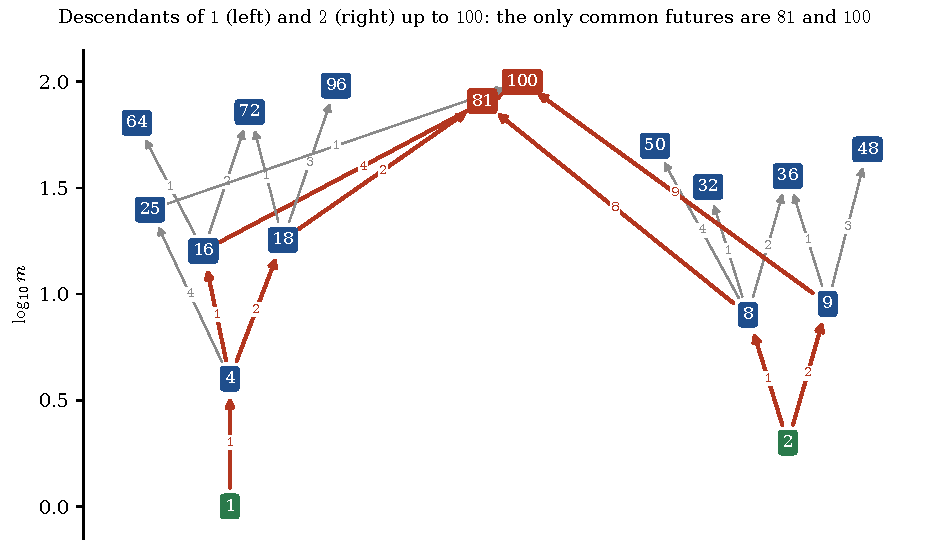
\includegraphics[width=\linewidth]{figs/fig_nojoin.pdf}
\caption{Proof of Theorem~\ref{thm:nojoin}. Vertices are placed at height \(\log_{10}m\); edge labels are the divisors \(N\). Red: the four paths from \(1\) and \(2\) to the common futures \(81\) and \(100\). Since \(81\) cannot reach \(100\), the pair \((1,2)\) has two incomparable minimal common futures and no least one.}\label{fig:nojoin}
\end{figure}

\begin{proposition}[Failure of general meets]\label{prop:nomeet}
\scope{A2}\record{S2.7} The order is not a meet-semilattice. In particular the pair \((32,300)\) has two distinct incomparable maximal common ancestors \(2\) and \(6\), as recorded by the exact finite predecessor computation of SELECT-II v002.
\end{proposition}
\begin{proof}
Every backward edge divides the vertex by at least four, so ancestor sets are finite and are computed by the recursion of Theorem~\ref{thm:reach-rec}, using \(\Pred(t)=\{(t/d^2)(d-1):d\in\Dx(t)\}\). For \(32\): \(\Dx(32)=\{2,4\}\), so \(\Pred(32)=\{8,6\}\); \(\Pred(8)=\{2\}\); \(\Pred(2)=\Pred(6)=\varnothing\). For \(300\): \(\Dx(300)=\{2,5,10\}\), so \(\Pred(300)=\{75,48,27\}\); further \(\Pred(75)=\{12\}\), \(\Pred(48)=\{12,9\}\), \(\Pred(27)=\{6\}\), \(\Pred(12)=\{3\}\), \(\Pred(9)=\{2\}\), and \(3,6,2\) have no predecessors. Hence
\[
 \mathrm{Anc}(32)=\{2,6,8,32\},\qquad
 \mathrm{Anc}(300)=\{2,3,6,9,12,27,48,75,300\},
\]
and the common ancestors are \(\{2,6\}\). Neither reaches the other: a nontrivial path multiplies the starting value by at least \(4\), but \(6/2=3<4\) and \(2/6<1\). Both are therefore maximal common ancestors. A greatest lower bound of \(32\) and \(300\) would be a common ancestor lying above every common ancestor, hence above both \(2\) and \(6\); by maximality it would equal \(2\) and also equal \(6\), which is impossible.
\end{proof}
\begin{figure}[t]
\centering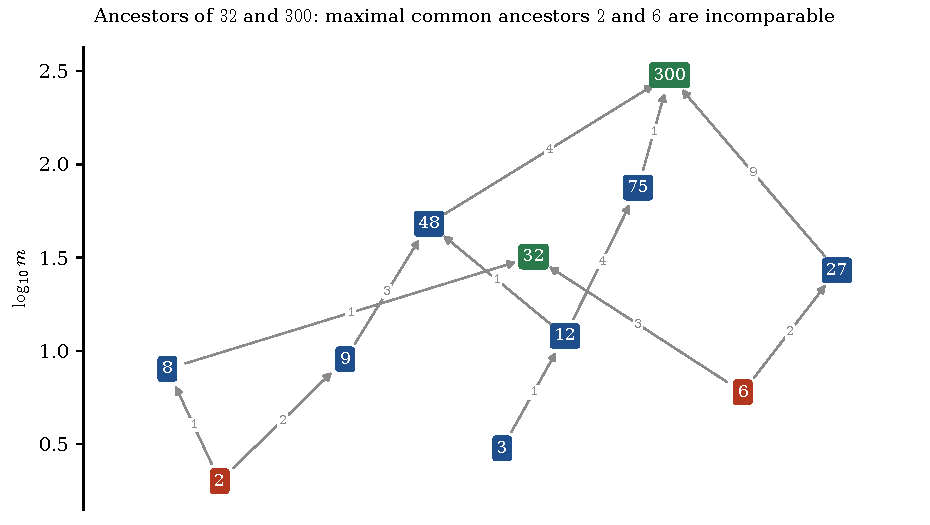
\includegraphics[width=\linewidth]{figs/fig_meets.pdf}
\caption{Proof of Proposition~\ref{prop:nomeet}: the ancestors of \(32\) and \(300\). The common ancestors \(2\) and \(6\) (red) are incomparable, so there is no greatest common ancestor.}\label{fig:meets}
\end{figure}

\begin{proposition}[The route join is not a successor-order object: a certificate]\label{prop:joinintr}
\scope{A2}\record{S2.8} In \(\Fx(72)\) take the anchor routes \(r=(18,2)\) and \(s=(8,3)\) (indices \(2\) and \(3\)). Their predecessor vertices are \(18\) and \(16\). The componentwise join \(\join(r,s)=(72,6)\) has value \(72\cdot6^2=2592\). Then \(2592\) is not reachable from \(72\), nor from \(18\) (it is reachable from \(16\)). In particular it is not a common future of the two predecessors of the routes, and the arithmetic of \(\join\) is not recovered from the order of Chapter~\ref{ch:graph}.
\end{proposition}
\begin{proof}
The join is \((\lcmop(18,8),\lcmop(2,3))=(72,6)\), of value \(72\cdot36=2592\). By Theorem~\ref{thm:reach-rec} membership in the ancestor set of \(2592\) is decided by backward recursion. \(\Dx(2592)=\{2,3,4,6,9,12,18,36\}\) gives \(\Pred(2592)=\{648,576,486,360,256,198,136,70\}\). Continuing the recursion, the ancestor set of \(2592\) has exactly \(42\) elements, among them \(16\), but neither \(72\) nor \(18\) (nor \(10\)); the full list is reproduced by the verifier \texttt{check\_volume\_i.py}.
\end{proof}
This is a single exact certificate. The source's counts over larger samples remain data and are not used here.

The registry also records extensive counts of finite no-join and no-meet witnesses. Their counts describe the enumerated sample; the counterexamples above, not the population percentages, establish the non-semilattice conclusions.

\chapter{Histories, Hasse Structure, and the Markov No-Go}\label{ch:histories}
\section{Backward recurrence and an exact decision procedure}
\begin{definition}[Ancestry and full histories]
For \(t\in\N_{>0}\), let \(\Pred(t)\) be the set of its incoming predecessor vertices. A \emph{complete history} of \(t\) is an edge-labelled directed path from a squarefree source to \(t\), with the length-zero history at a source counted once. Let \(\nohist(t)\) count these paths.
\end{definition}

\begin{theorem}[Backward reachability recurrence]\label{thm:reach-rec}
\scope{A2}\record{S2.9} For positive integers \(m\le t\),
\begin{equation}\label{eq:reachrec}
 m\rightsquigarrow t\iff m=t\quad\text{or}\quad
 \exists p\in\Pred(t):m\rightsquigarrow p.
\end{equation}
The recurrence terminates, and every path from \(m\) to \(t\), when \(m<t\), has length at most \(\lfloor\log_4(t/m)\rfloor\).
\end{theorem}
\begin{proof}
Any nonempty path into \(t\) has a last edge \(p\to t\), so removing that edge gives the recursive alternative. The converse is obtained by appending it. Theorem~\ref{thm:degrees} gives \(p\le t/4\), so the backward recursion strictly decreases. A path of \(j\) edges multiplies its initial value by at least \(4^j\), yielding \(4^j m\le t\).
\end{proof}
\begin{corollary}[Decidability of reachability]\label{cor:decide}
\scope{A2}\record{S2.6} For given integers \(m\le t\) the relation \(m\rightsquigarrow t\) is decided by a terminating procedure: compute \(\Pred(t)\) from the square divisors of \(t\), recurse on each predecessor that is at least \(m\), and accept as soon as \(m\) is met. The recursion visits only integers in \([m,t]\), at depth at most \(\lfloor\log_4(t/m)\rfloor\).
\end{corollary}
\begin{proof}
This is Theorem~\ref{thm:reach-rec} read as an algorithm. Predecessors of a vertex are at most one quarter of it, so predecessors below \(m\) cannot lead back to \(m\) and may be discarded; every visited vertex lies in \([m,t]\), so the search is finite.
\end{proof}
This settles decidability, not the open problem of a closed-form criterion (Appendix~\ref{app:open}).

\begin{theorem}[No shortcuts: the graph is the Hasse diagram]\label{thm:hasse}
\scope{A2}\record{S2.10} If \(p\to t\) is a direct edge, then no path of two or more edges goes from \(p\) to \(t\). Thus every graph edge is a cover relation, and \(\Gen\) is the Hasse diagram of the reachability order. In particular, distinct predecessors of one target are pairwise incomparable.
\end{theorem}
\emph{Idea.} A shortcut would mean that the single multiplier \(d^2/(d-1)\) factors into two or more multipliers of the same kind. Comparing numerators and denominators leaves one integer equation whose two sides have incompatible sizes.
\begin{proof}
Writing a direct-edge multiplier with \(d=N+1\), we have \(\varphi(d)=d^2/(d-1)\). Suppose that the same ratio of target to source can be expressed as a product of \(j\ge2\) edge multipliers \(\varphi(d_i)\). Then
\[
 \frac{d^2}{d-1}=\prod_{i=1}^j\frac{d_i^2}{d_i-1},\qquad
 (d-1)\Big(\prod_i d_i\Big)^2=d^2\prod_i(d_i-1).
\]
Since \(\gcdop(d,d-1)=1\), the latter equation forces \(d\mid\prod_i d_i\) and \((d-1)\mid\prod_i(d_i-1)\). Write
\[
 \prod_i d_i=da,\qquad\prod_i(d_i-1)=(d-1)b,
\]
with positive integers \(a,b\). The displayed equality implies \(b=a^2\), hence
\begin{equation}\label{eq:noshortcut}
 \prod_i d_i-\prod_i(d_i-1)=a\big(d-(d-1)a\big).
\end{equation}
The left-hand side is at least three for \(j\ge2\) and \(d_i\ge2\). If \(a=1\), the right side is one; if \(a\ge2\), it is nonpositive. Both cases contradict the positivity and lower bound of the left-hand side. Hence no shortcut exists. Every edge is a cover by definition; conversely if \(p\rightsquigarrow t\) is a cover, any path realizing it must have length one, so it is an edge. Finally, a path between two different predecessors would combine with their edges to \(t\) to create a forbidden shortcut.
\end{proof}

\begin{remark}[The graph is not graded]\label{rem:graded}
\scope{A2}\record{S2.11} The source records paths of both two and three edges from 6 to 784. Thus path length is not a well-defined rank difference, even though every edge is a cover. The fact is certified by a finite explicit example, not a general assertion about all intervals.
\end{remark}
\begin{figure}[t]
\centering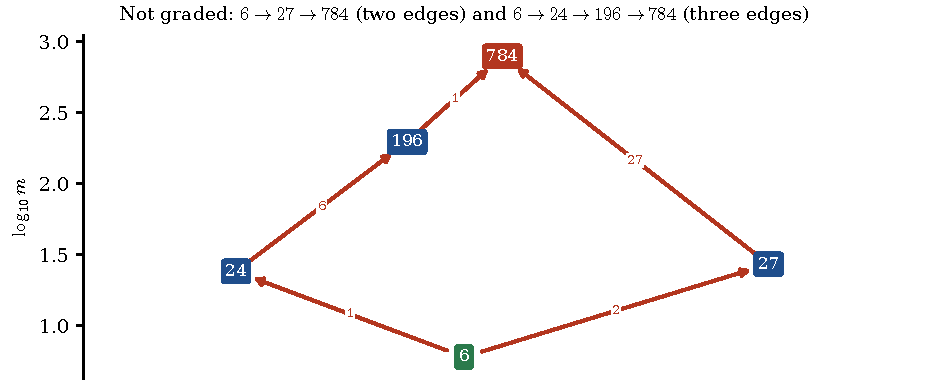
\includegraphics[width=\linewidth]{figs/fig_notgraded.pdf}
\caption{Remark~\ref{rem:graded}: two paths from \(6\) to \(784\) of different lengths, although every edge is a cover relation.}\label{fig:notgraded}
\end{figure}

\section{Endpoint multiplicity versus history multiplicity}
\begin{theorem}[Complete-history recurrence]\label{thm:hist-rec}
\scope{A2}\record{S2.12} The number of complete histories satisfies
\begin{equation}\label{eq:history}
 \nohist(t)=\begin{cases}1,&\Pred(t)=\varnothing,\\
 \displaystyle\sum_{p\in\Pred(t)}\nohist(p),&\Pred(t)\ne\varnothing.
 \end{cases}
\end{equation}
For every non-source, \(\nohist(t)\ge R(t)\), with equality if and only if each immediate predecessor has precisely one complete history.
\end{theorem}
\begin{proof}
For a source the only complete history is the trivial one. Otherwise every complete history ends with exactly one incoming edge \(p\to t\). These disjoint sets of histories are counted by the right side of \eqref{eq:history}; the recursion is finite by strict descent. There are \(R(t)\) distinct predecessors by Theorem~\ref{thm:pred}, and each has at least one history. Equality of their sum with \(R(t)\) holds precisely when all summands equal one.
\end{proof}

\begin{example}[Four histories ending at a three-route value]
For \(t=72\), the complete paths are
\[
 1\to4\to18\to72,\quad
 1\to4\to16\to72,\quad
 3\to16\to72,\quad
 10\to72.
\]
Thus \(\nohist(72)=4\) whereas \(R(72)=3\). The incoming route through predecessor 16 admits two different earlier histories. This supplies a strict hierarchy: the numerical endpoint is one object, the entering route adds information, and the complete history may add still more.
\end{example}
\begin{figure}[t]
\centering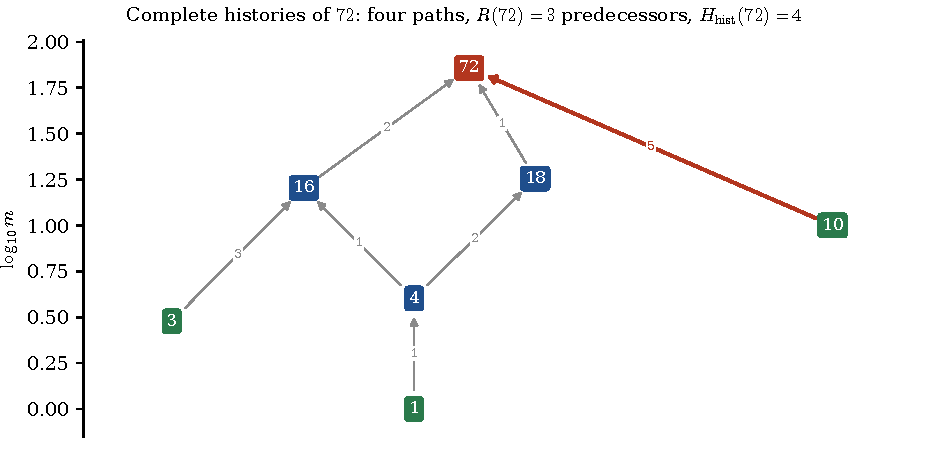
\includegraphics[width=\linewidth]{figs/fig_hist72.pdf}
\caption{The ancestry of \(72\) (Example~\ref{ex:72}). Sources \(1\), \(3\), \(10\) are squarefree (green). Three edges enter \(72\); the edge from \(16\) carries two different earlier histories (\(1\to4\to16\) and \(3\to16\)), giving four complete histories.}\label{fig:hist72}
\end{figure}

\section{Why forward continuation does not read the past}
\begin{theorem}[Endpoint Markov property]\label{thm:markov}
\scope{A2}\record{S2.13} In the declared self-substitution graph, the set of possible forward extensions of any finite history depends only on its terminal vertex. In particular, a joint construction that is defined solely by forward graph extension and that observes only the endpoint of a merger cannot distinguish two histories with the same endpoint.
\end{theorem}
\begin{proof}
By Definition~\ref{def:graph}, the allowable outgoing edges from a vertex \(t\) are determined solely by the divisors of \(t\). They do not depend on the path by which \(t\) was reached. Iterating this observation proves equality of all future descendant sets for histories sharing endpoint \(t\). An endpoint-only merger observation is a function of those future descendant sets and so is identical for such histories.
\end{proof}

\begin{remark}[Nature of the no-go theorem]
The proof is short because the content is a modelling statement rather than a deep calculation: the graph \(\Gen\) is memoryless by construction, so any observation that factors through the forward graph from the endpoint cannot see the past. What carries mathematical weight is the contrast with Theorem~\ref{thm:hist-rec}, which shows that the past is nevertheless nontrivial (\(\nohist(t)>R(t)\) can occur).
\end{remark}

\begin{remark}[Precise limitation of the no-go theorem]
The theorem does not forbid history-sensitive structures constructed with additional state variables, retrospective ancestry operators, labelled memories or different observation maps. It says only that the \emph{forward endpoint semantics of A2} does not expose history. A different generative grammar can be developed and analyzed, but its new state or operation must be given explicitly.
\end{remark}

\begin{proposition}[Predecessor-input leakage]\label{prop:leak}
\scope{A2}\record{S2.14} For distinct incoming routes \(r,s\) to the same target \(t\), their respective predecessor vertices \(p(r),p(s)\) are incomparable. A probe that directly includes these predecessor values can therefore distinguish the routes without measuring any forward interaction of the two routes.
\end{proposition}
\begin{proof}
Predecessor incomparability is Theorem~\ref{thm:hasse}. Reading the predecessor vertex is, by construction, reading data that already differentiates distinct incoming edges. The source's \(J_{\mathrm{pred}}\) calculation operationalizes precisely this leakage; its finite statistics are not needed for the logical conclusion.
\end{proof}

\begin{proposition}[Minimal confluence at every target]\label{prop:confluence}
\scope{A2}\record{S2.15} For two distinct incoming predecessors \(p,p'\) of a target \(t\), the target \(t\) is a minimal common future of \(p,p'\). This need not make \(t\) their unique minimal common future.
\end{proposition}
\begin{proof}
It is a common future by the two incoming edges. If some common future \(u\ne t\) satisfied \(u\rightsquigarrow t\), then \(p\rightsquigarrow u\rightsquigarrow t\) would give a shortcut to the direct edge \(p\to t\), contradicting Theorem~\ref{thm:hasse}. Hence \(t\) is minimal. The source exhibits exact finite examples with two incomparable minimal common futures, including the case of routes entering \(784\), for which \(432\) and \(784\) are both minimal.
\end{proof}

\section{Open classification questions}
Three distinct problems remain open in the registry for this chapter: a nonrecursive number-theoretic reachability criterion for \(m\rightsquigarrow t\); a systematic description of multi-minimal confluence and the observed exceptional pairs; and a substantive relationship, if any, between retrospective merge invariants and the distance from the earlier relational-invariants manuscript. The exact backward recurrence proves \emph{decidability}, not the sought closed-form criterion. No physical entanglement mechanism is claimed here.

\chapter{Admissibility, Interaction Nonselection, and Incompatibility}\label{ch:nonselection}
\section{From common futures to an interaction specification}
Chapters~\ref{ch:rendezvous}--\ref{ch:histories} specify arithmetic and two alternative generative interpretations. Their results do not provide a distinguished binary interaction. To formulate the selection problem, let
\[
 \operatorname{Dom}=\{(r,s):r,s\in\Fx(x)\text{ for some }x,\ r\ne s\}.
\]
A \emph{value-valued interaction candidate} is a map \(\star:\operatorname{Dom}\to\Q_{>0}\). We state the relevant axioms precisely, so that statements of consistency or incompatibility have an identifiable domain.

For \(r,s\in\Fx(x)\), let \(\tau_i(r,s)\) be the ordered pair obtained by advancing both fixed-index routes from \(x\) to \(x+i\Del_{rs}\), where \(i\ge0\). Let \(\Pi=\prod_x\operatorname{Sym}(\Fx(x))\) be the group of independent permutations of each occurrence fibre.

\begin{definition}[Interaction axioms]\label{def:axioms}
For a value-valued candidate \(\star\) define:
\begin{description}[style=nextline,leftmargin=2em]
\item[Symmetry (Sym)] \(r\star s=s\star r\).
\item[Common-future admissibility (CF)] \(r\star s\in x+\Del_{rs}\Z_{\ge1}\).
\item[Stationarity (Stat)] \(\tau_i(r,s)_1\star\tau_i(r,s)_2-(x+i\Del_{rs})=r\star s-x\) for all \(i\ge0\).
\item[Label-blindness (LB)] \((\pi r)\star(\pi s)=r\star s\) for all \(\pi\in\Pi\).
\item[Weak partner independence (LBw)] For pairwise distinct \(r,s,t\in\Fx(x)\), one has \(r\star s=r\star t\).
\item[Pair minimality (PMin)] \(r\star s=x+\Del_{rs}\).
\item[Collective minimality (CMin)] \(r\star s=x+\Del_{\mathrm{coll}}(x)\).
\end{description}
The axiom labels Sym, CF, Stat, LB, LBw, PMin, CMin replace the labels A2, A3, A4, A6, A6w, A7p, A7c used in the source records, which would collide with the scope labels A0, A1, A2 of this volume. Each axiom is a proposed constraint on an interaction, not an automatic consequence of the arithmetic construction. In particular, LB implies LBw, but not conversely as a formal logical condition.
\end{definition}

\begin{proposition}[The labelled structure carries exactly the label]\label{prop:labelled}
\scope{X}\record{F.T10} Call \(\operatorname{Occ}=\N_{>0}^2\) the set of occurrences \((M,N)\), with value \(v(M,N)=M(N+1)^2/N\) and routes \(\{(M,N):M\ge1\}\) for each fixed \(N\). (a) The map \(r\mapsto(v(r),v(F r))\) is injective. (b) The structure \((\operatorname{Occ},v,\text{route membership})\) has trivial automorphism group: a bijection of \(\operatorname{Occ}\) that preserves values and maps routes onto routes is the identity.
\end{proposition}
\begin{proof}
(a) The step \(v(Fr)-v(r)=(N+1)^2/N\) is a reduced fraction because \(\gcdop(N,(N+1)^2)=1\); its denominator is \(N\). Hence \(N\) is recovered from the pair, and then \(M=v(r)N/(N+1)^2\).
(b) Let \(\varphi\) be such a bijection. It maps route \(N\) onto some route \(N'\) and preserves values, so the two routes have the same value set. The value set of route \(N\) is \(\{M(N+1)^2/N:M\ge1\}\) with least element \(\sigma_N=N+2+1/N\), which is strictly increasing in \(N\). So \(N'=N\). Within a route the values \(M\sigma_N\) are pairwise distinct, so \(\varphi\) fixes each occurrence.
\end{proof}
Consequently any invariant that retains route membership is equivalent to the label \((M,N)\); a label-blind structure can only be a structure on values, whose symmetry is the group \(\Pi\). This is why label-blindness is formulated through \(\Pi\) below. (The source records the claim in (b) with a finite check; the argument above makes it a proof.)

\section{The nonselection theorems}
\begin{theorem}[All admissible pair-value outputs]\label{thm:star-family}
\scope{X}\record{F.T12, Theorem N} An operation satisfying common-future admissibility has the form
\begin{equation}\label{eq:family}
 r\star s=x+j(r,s)\Del_{rs},\qquad j(r,s)\in\N_{>0}.
\end{equation}
Symmetry holds if and only if \(j\) is symmetric; stationarity holds if and only if \(j\) is constant along every \(\tau\)-orbit. There are infinitely many such operations. Pair minimality selects \(j\equiv1\), but that is an additional constraint.
\end{theorem}
\begin{proof}
Theorem~\ref{thm:pair} characterizes the common future values of the two routes; excluding their present value \(x\) yields \eqref{eq:family}. Its step \(\Del_{rs}\) is symmetric and remains the same under joint translation of the fixed-index routes. Thus symmetry and stationarity impose exactly the respective conditions on the positive integer selector \(j\). Every constant function \(j\equiv c\ge1\) satisfies these conditions; constants \(c\ne c'\) give different operations. The first positive common future is precisely \(c=1\).
\end{proof}

\begin{lemma}[Orbit lemma]\label{lem:orbit}
\scope{X}\record{F.T11} On a fibre \(\Fx(x)\) with \(R(x)\ge2\), the group \(\operatorname{Sym}(\Fx(x))\) acts transitively on the unordered pairs of distinct occurrences. Hence a \(\Pi\)-invariant function of an unordered pair is a function of the fibre alone.
\end{lemma}
\begin{proof}
Given unordered pairs \(\{r,s\}\) and \(\{r',s'\}\) of distinct elements, the permutation of \(\Fx(x)\) sending \(r\mapsto r'\), \(s\mapsto s'\) (extended arbitrarily) maps one to the other.
\end{proof}

\begin{theorem}[Label-blind candidates are value-valued operations factoring through the fibre value]\label{thm:blind}
\scope{X}\record{F.T11, F.T13} Any value-valued \(\star\) satisfying Sym, CF and LB must be of the form
\begin{equation}\label{eq:blind}
 r\star s=Y(x)=x+j(x)\Del_{\mathrm{coll}}(x),\qquad j(x)\in\N_{>0}.
\end{equation}
Conversely any choice of such \(j(x)\) defines a label-blind symmetric admissible operation. The minimal collective choice is \(Y_1(x)=x+\Del_{\mathrm{coll}}(x)\).
\end{theorem}
\begin{proof}
By Lemma~\ref{lem:orbit}, on a fixed fibre the group \(\operatorname{Sym}(\Fx(x))\) acts transitively on unordered pairs of distinct occurrences. Symmetry and label-blindness force the output to have one value \(Y(x)\) for every such pair. Common-future admissibility requires that \(Y(x)-x\) be a positive multiple of each \(\Del_{rs}\), hence of their lattice-lcm \(\Del_{\mathrm{coll}}\). The converse follows from this characterization and the fact that the right side depends only on \(x\).
\end{proof}

\begin{remark}[A necessary correction to a common reading]\label{rem:gamma}
The arithmetic invariant \(\gamma(x)=x/\Del_{\mathrm{coll}}(x)\) controls the set of allowed collective increments; it does \emph{not} force the freely chosen selector \(j(x)\) to depend only on \(\gamma\). For example \(Y(x)=2x\) corresponds to \(j(x)=\gamma(x)\). Other selectors may use any additional fibre invariant or no invariant at all. This is the recorded v003 clarification to earlier ``only gamma matters'' wording.
\end{remark}

\begin{theorem}[Incompatibility of stationarity and weak label-blindness]\label{thm:incompat}
\scope{X}\record{F.T15, Theorem I} On the full domain \(\operatorname{Dom}\), there exists no value-valued operation satisfying simultaneously CF (common-future admissibility), Stat (stationarity along all pair shifts), and LBw (weak partner independence). Therefore CF, Stat and the stronger LB are also incompatible.
\end{theorem}
\emph{Idea.} Stationarity forces the output gap \(P=r\star s-x\) to be one fixed rational for all shifts. Moving along the common-future progression we can reach a value whose fibre acquires a brand-new index \(p\), a large prime; weak partner independence then ties the output to a pair involving \(p\), whose admissible gaps all carry a factor \(p^2\). A single fixed number cannot be divisible by \(p^2\) for infinitely many primes.
\begin{proof}
Fix a pair \(r\ne s\in\Fx(x)\) for \(x=a/b\) reduced. Let their indices be \(d,d'\), set \(N=d-1\), \(N'=d'-1\), \(g_{rs}=\gcdop(N,N')\), \(L=\lcmop(d,d')\), and \(\Del=L^2/g_{rs}\). By Theorem~\ref{thm:pairindex}, \(b\mid g_{rs}\). Its paired shifts have common value
\[
 y_i=x+i\Del=\frac{a g_{rs}/b+iL^2}{g_{rs}},\qquad i\ge0.
\]
Choose any prime \(p>\max(g_{rs},L)\) with \(p\equiv1\pmod{g_{rs}}\). There are infinitely many such primes by Dirichlet's theorem. Since \(p\nmid L\), there is an integer \(i\ge0\) with \(a g_{rs}/b+iL^2\equiv0\pmod{p^2}\). Write \(y_i=u/e\) in reduced form; then \(p^2\mid u\), \(e\mid g_{rs}\), and \(e\mid(p-1)\). Consequently
\[
 q=\left(\frac{u(p-1)}{e p^2},p-1\right)
\]
is an occurrence of \(y_i\) with index \(p\). It differs from the two fixed-index shifts \(r_i,s_i\), since \(p>L\ge d,d'\). Hence \(r_i,s_i,q\) are three distinct occurrences at \(y_i\).

By LBw, \(r_i\star s_i=r_i\star q=:Y_i\). By CF applied to the latter pair, the positive gap \(P_i=Y_i-y_i\) is a multiple of
\[
 \Del_{r_iq}=\frac{\lcmop(d,p)^2}{\gcdop(d-1,p-1)}
 =\frac{d^2p^2}{\gcdop(d-1,p-1)}.
\]
Its reduced numerator is divisible by \(p^2\), as \(p\) divides neither \(d\) nor the displayed gcd. By Stat applied to the original pair, however, \(P_i=r\star s-x=:P\), a single \emph{fixed positive rational} independent of \(i\) and \(p\). Its reduced numerator cannot be divisible by \(p^2\) for infinitely many distinct primes \(p\). This contradiction completes the proof.
\end{proof}

\begin{remark}[Exact scope of Theorem~\ref{thm:incompat}]
The argument uses unrestricted common-future shifts for a fixed pair, partner-independence on the larger fibres reached, and a \emph{value-valued} output. It does not rule out restrictions to smaller domains or to prescribed shifts, fibre-valued outputs, or invariance under proper subgroups of \(\Pi\). Nor does it make the collective choice necessary; it proves the incompatibility of two proposed invariances on the full domain.
\end{remark}

\begin{theorem}[No fully equivariant occurrence selector]\label{thm:noselector}
\scope{X}\record{F.T14} There is no \(\Pi\)-equivariant operation assigning to each pair of distinct same-value occurrences an individual occurrence in their strict common future.
\end{theorem}
\begin{proof}
Suppose the output is an occurrence at \(y>x\). The fibre \(\Fx(y)\) contains the two distinct continued occurrences, so it has at least two elements. A permutation of \(\Fx(y)\) may exchange the proposed output occurrence with another while fixing every occurrence in \(\Fx(x)\), because \(y\ne x\) and \(\Pi\) independently permutes fibres. Equivariance would require this permutation to fix the output, a contradiction.
\end{proof}

\section{Declared grammars and the bridge to Volume II}\label{sec:declared}
There are two especially transparent candidates:
\begin{enumerate}[label=(\roman*)]
\item \emph{Route-aware pair continuation} \(r\star_j s=x+j\Del_{rs}\). With constant \(j\), this satisfies symmetry, common-future admissibility and stationarity, but not general label-blindness.
\item \emph{Collective value continuation} \(C(x)=x+\Del_{\mathrm{coll}}(x)=x+L(x)^2/G(x)\). It satisfies label-blindness and collective minimality but is generally nonstationary in the above pair-shift sense.
\end{enumerate}
Neither option is uniquely mandated by the arithmetic rule \eqref{eq:base}, and neither is a universal consequence of SELECT-II's reachability graph. Figure~\ref{fig:axioms} summarises which combinations of axioms are realisable. Volume II will study the second, \(C\), by explicit adoption of that grammar. Its theorems on fibre growth, exact eventual scaling, single-prime rigidity and effective transient bounds are consequences of \(C\), not of a logically forced continuation from Volume I.

\begin{figure}[t]
\centering
\begin{tikzpicture}[>=Stealth,x=1cm,y=1cm]
\node[box,text width=5.4cm] (base) at (0,3.0) {Sym + CF\\ (symmetric, lies in the common future)};
\node[box,fill=green!10,text width=4.7cm] (l) at (-3.7,0.7) {+ Stat: $r\star s=x+j(r,s)\Delta_{rs}$, any $j$ constant on orbits: \emph{infinite family} (Thm~\ref{thm:star-family})};
\node[box,fill=green!10,text width=4.7cm] (r) at (3.7,0.7) {+ LB: $r\star s=Y(x)=x+j(x)\Delta_{\mathrm{coll}}$, value-valued, $j(x)$ free (Thm~\ref{thm:blind})};
\node[box,fill=red!10,text width=5.6cm] (b) at (0,-1.7) {Stat + LBw together:\\ \textbf{no operation exists} (Thm~\ref{thm:incompat})};
\node[box,fill=red!10,text width=7.2cm] (o) at (0,-3.5) {Occurrence-valued and $\Pi$-equivariant: \textbf{none} (Thm~\ref{thm:noselector})};
\draw[->] (base) -- (l); \draw[->] (base) -- (r);
\draw[->] (l) -- (b); \draw[->] (r) -- (b);
\end{tikzpicture}
\caption{Which axiom combinations can be realised. Green: realisable, with the form of all solutions. Red: impossible. LB implies LBw, so adding LB to Stat is also impossible.}\label{fig:axioms}
\end{figure}

\section{Principal conclusions of Volume I}
We have established, within stated and distinct domains, the following hierarchy: arithmetic realization determines a finite fibre; pair and collective common futures determine lattices of admissible values; a componentwise amplification order gives one join, while adding refinement changes the continuation; a self-substitution graph gives an acyclic, nongraded reachability order without universal meets or joins; full histories contain information that endpoint-only forward continuation does not reveal; and value-valued label-blindness conflicts with stationarity over the full common-future domain.

The fundamental result is therefore neither ``interaction does not exist'' nor ``one interaction has been derived.'' The precise mathematical statement is \emph{nonselection}: specified arithmetic and consistency constraints do not suffice to distinguish one joint-operation grammar. This conclusion leaves room for additional, explicitly constructed UNNS grammar and provides the proper logical entry to the dynamical results of the companion volume.

\appendix
\chapter{Theorem identification and scopes}\label{app:crosswalk}
The source registry contains 128 records across the coordinated volumes; 60 are assigned to Volume I. The crosswalk below identifies those 60 records by the registry's original IDs. It distinguishes archived proof labels from an independent proof audit. Not all 60 source records receive stand-alone re-proofs in this edition: the principal structural arguments appear in the seven chapters, while auxiliary cases, computational comparisons, open questions and historical corrections remain directly traceable through their original records. The original archived statements and limitations take precedence over abbreviated crosswalk titles. Titles in the table are quoted from the registry and keep the source axiom labels (A1--A7); in the body these are renamed Sym, CF, Stat, LB, LBw, PMin, CMin (Section~7.1). Record S2.7 is registered as DATA because its source reports counts over enumerated samples; Proposition~\ref{prop:nomeet} is a different statement, a single exact counterexample with its ancestor sets listed, and is therefore proved here, while the counts remain DATA.

Three separate SELECT-II source lines retain their published directory paths. The labels \emph{v001} (base), \emph{v002a} (the directory named \texttt{v002}) and \emph{v002b} (the distinct continued line) are editorial labels only. The original source files are not renamed.

\footnotesize
\begin{longtable}{@{}p{16mm}p{59mm}p{38mm}p{13mm}@{}}
\toprule
Registry ID & Source record title & Source status & Scope\\\midrule
\endfirsthead
\toprule Registry ID & Source record title & Source status & Scope\\\midrule
\endhead
\texttt{F.T1} & Rational-Fibre Theorem & PROVED+CHECKED & A0 \\
\texttt{F.T16} & Join on rational fibres (corrected T4) & PROVED+CHECKED & A0 \\
\texttt{F.T1p} & Reparametrisation & PROVED+CHECKED & A0 \\
\texttt{F.T1pp} & Sub-fibre form & PROVED & A0 \\
\texttt{F.T22} & Reduction to the square-root part & PROVED+CHECKED & A0 \\
\texttt{F.T3} & Realisability & PROVED & A0 \\
\texttt{F.T4} & Congruence obstruction (original form) & CORRECTED & A0 \\
\texttt{F.T5} & Refinement preserves the rational fibre & PROVED & A0 \\
\texttt{F.F5} & Rendezvous x+L\textasciicircum{}2/gcd(N,N') (v001 observation) & DATA & A0 \\
\texttt{F.L0} & Lattice lcm (Lemma 0) & PROVED & A0 \\
\texttt{F.T2} & Cross-nest intersection & PROVED & A0 \\
\texttt{F.T6} & Common future of a pair & PROVED+CHECKED & A0 \\
\texttt{F.T7} & Integrality of the rendezvous index & PROVED+CHECKED & A0 \\
\texttt{F.T8} & Collective rendezvous, coherence, gamma=gcd H & PROVED+CHECKED & A0 \\
\texttt{F.T9} & Every positive integer is a pair index & PROVED+CHECKED & A0 \\
\texttt{F.T20} & Integer R=3 fibres are non-rigid & PROVED+CHECKED & A0 \\
\texttt{F.T21} & Rigid rational R=3 example & CHECKED & A0 \\
\texttt{F.T23} & Closure lemmas (Q), (G) & PROVED+CHECKED & A0 \\
\texttt{F.T24} & Shape theorem for three-route fibres (b>=2) & PROVED+CHECKED & A0 \\
\texttt{F.T25} & Infinite rigid families & PROVED & A0 \\
\texttt{F.T29} & Signature criterion for three-route rigidity & PROVED+CHECKED & A0 \\
\texttt{O4.1} & Fibre classification, R-growth rate, branch comparison & OPEN & MIXED \\
\texttt{O.S1} & SELECT-I: justification of E, T\_q status, retention & OPEN & A1 \\
\texttt{S1.1} & Selection = reachability order & PROVED & A1 \\
\texttt{S1.2} & Coordinate rigidity & PROVED+CHECKED & A1 \\
\texttt{S1.3} & Amplification order and J\_join & PROVED+CHECKED & A1 \\
\texttt{S1.4} & Minimality from absorption & PROVED & A1 \\
\texttt{S1.5} & Fork: refinement as a generative step & PROVED+CHECKED & A1 \\
\texttt{S1.6} & Nest iteration consumes the factor N & PROVED+CHECKED & A1 \\
\texttt{S1.7} & Discrimination matrix of joint operations & CHECKED & A1 \\
\texttt{S1.8} & SELECT-I verdict (S5) & INTERPRETATION & A1 \\
\texttt{S2.1} & Out-degree, growth and acyclicity & PROVED & A2 \\
\texttt{S2.2} & In-degree equals nest multiplicity & PROVED & A2 \\
\texttt{S2.3} & Edge label is identifiable & PROVED & A2 \\
\texttt{S2.4} & No universal least common future & PROVED & A2 \\
\texttt{S2.5} & Occurrence = edge; fibre multiplicity = in-degree & PROVED+CHECKED & A2 \\
\texttt{S2.6} & Fixed-target reachability is decidable & PROVED & A2 \\
\texttt{S2.7} & Joins and meets fail (counts) & DATA & A2 \\
\texttt{S2.8} & J\_join is not an intrinsic reachability object & DATA & A2 \\
\texttt{O.S2a} & SELECT-II: closed-form criterion for m ~> t & OPEN & A2 \\
\texttt{O.S2b} & SELECT-II: double-confluence pattern and Min C(a,b) & OPEN & A2 \\
\texttt{O.S2c} & SELECT-II: retrospective invariants vs D & OPEN & A2 \\
\texttt{S2.10} & No shortcuts: every edge is a cover relation & PROVED+CHECKED & A2 \\
\texttt{S2.11} & Path length is not a rank function & CHECKED & A2 \\
\texttt{S2.12} & History counts H(t) & PROVED+CHECKED & A2 \\
\texttt{S2.13} & Markov no-go for continuation & PROVED+CHECKED & A2 \\
\texttt{S2.14} & J\_pred separates automatically (leakage) & PROVED+CHECKED & A2 \\
\texttt{S2.15} & Intrinsic confluence of fibre routes & PROVED+CHECKED & A2 \\
\texttt{S2.16} & SELECT-II verdict & INTERPRETATION & A2 \\
\texttt{S2.9} & Backward recurrence for reachability & PROVED+CHECKED & A2 \\
\texttt{F.E3} & Erratum: 'only gamma matters' (v003) & CORRECTED & X \\
\texttt{F.G1R} & G1-R route-aware pair interaction & PROPOSED & R \\
\texttt{F.GI} & Theorem I (A3+A4+A6w incompatible) & PROVED+CHECKED & X \\
\texttt{F.GN} & Theorem N (nonselection among A2+A3 operations) & PROVED+CHECKED & X \\
\texttt{F.T10} & Rigidity of the labelled structure & PROVED+CHECKED & X \\
\texttt{F.T11} & Regime A / orbit lemma & PROVED+CHECKED & X \\
\texttt{F.T12} & Admissible family (non-selection from A1-A3) & PROVED+CHECKED & X \\
\texttt{F.T13} & Label-blind operations are collective & PROVED+CHECKED & X \\
\texttt{F.T14} & No label-blind occurrence-valued operation & PROVED+CHECKED & X \\
\texttt{F.T15} & Incompatibility of stationarity and label-blindness & PROVED+CHECKED & X \\
\bottomrule
\end{longtable}
\normalsize
\chapter{Reproducibility and bounded certificates}\label{app:checks}
The accompanying standalone Python script \texttt{check\_volume\_i.py} checks exact finite instances of the definitions and graph theorems using integer arithmetic only. Its checks are \emph{consistency tests}. They neither replace the hand proofs nor independently certify all 60 registry records. It is supplied as manuscript support and has no write access to the frozen GitHub reference collection.

The following source distinctions should be maintained:
\begin{enumerate}
\item Rational-fibre and graph facts are proved by arithmetic; their bounded computations are auxiliary checks.
\item The no-join witness \((1,2)\) includes an exact finite search below a bound justified by strict growth; hence that \emph{specific counterexample} is deductively complete.
\item Finite sample counts of rigid fibres, confluence exceptions, and operation-comparison matrices are labelled \textsf{CHECKED} or \textsf{DATA} according to source status, not recast as universal theorems.
\item The join of anchor routes is conditional on the factor-amplification order. The self-substitution graph uses a different reachability order. Results from one are not substituted silently for results from the other.
\item Historical corrections remain visible. In particular F.T16 corrects an omitted index lower bound in F.T4; other FIELD-I v003 wording regarding \(\gamma\) is read using its subsequent explicit correction.
\end{enumerate}

The exact source files and verification programs can be located using the permanent reference links in the bibliography. The separate master registry preserves the dependency DAG and exposition sequence independently.

\chapter{Outstanding mathematical questions}\label{app:open}
Volume I deliberately leaves the following issues unresolved rather than treating numerical patterns as completed proofs:
\begin{enumerate}
\item Full arithmetic classification of primitive rigid rational fibres and their structures; a growth-rate question in registry record O4.1 belongs specifically to the adopted collective map of Volume II.
\item Independent justification of treating amplification \(E\) as a generating move, treating refinement as symmetry or continuation, or requiring retention (O.S1).
\item A closed-form, nonrecursive necessary-and-sufficient criterion for \(m\rightsquigarrow t\) in the integer self-substitution order (O.S2a).
\item Classification of multiple minimal confluences and the exceptional route-pair patterns (O.S2b).
\item Whether natural retrospective graph invariants have a meaningful nontrivial relationship to the earlier route metric (O.S2c).
\item Interaction choices beyond the full-domain value-valued axioms, such as subgroup invariances, restricted domains, fibre-valued outputs and genuinely history-sensitive additional grammar.
\end{enumerate}
The presence of open questions does not prevent developing the established theorems into a coherent mathematical treatise. Their correct scope is part of the mathematical account.

\chapter{Proof-completeness audit of the crosswalk records}\label{app:audit}
For each of the 60 records assigned to this volume, the table states where its content stands in the text and how complete the argument given here is. \emph{Full proof}: the statement and a complete proof are in the text. \emph{Exact computation}: the claim is a finite exact statement and its certificate is displayed or reproduced by the verifier. \emph{Not a theorem}: the record is DATA, an interpretation, a proposal, or an open problem and is reported as such. No record is left with only a pointer to an archived proof.
\footnotesize
\begin{longtable}{@{}p{15mm}p{33mm}p{36mm}p{36mm}@{}}
\toprule ID & Location & Completeness here & Remark\\\midrule\endfirsthead
\toprule ID & Location & Completeness here & Remark\\\midrule\endhead
\texttt{F.T1} & Thm~\ref{thm:fibre} & Full proof &  \\
\texttt{F.T16} & Thm~\ref{thm:join-fibre} & Full proof & corrected form of F.T4 \\
\texttt{F.T1p} & Prop.~\ref{prop:reparam} & Full proof &  \\
\texttt{F.T1pp} & Prop.~\ref{prop:reparam} & Full proof &  \\
\texttt{F.T22} & Thm~\ref{thm:sqrtpart} & Full proof &  \\
\texttt{F.T3} & Thm~\ref{thm:real} & Full proof &  \\
\texttt{F.T4} & Thm~\ref{thm:join-fibre} & Superseded & original form corrected by F.T16 \\
\texttt{F.T5} & Prop.~\ref{prop:refine} & Full proof & \\
\texttt{F.F5} & Thm~\ref{thm:pair} & Full proof & observation proved as part of F.T6 \\
\texttt{F.L0} & Lem.~\ref{lem:lcm} & Full proof & valuation proof \\
\texttt{F.T2} & Thm~\ref{thm:pair} & Full proof &  \\
\texttt{F.T6} & Thm~\ref{thm:pair} & Full proof &  \\
\texttt{F.T7} & Thm~\ref{thm:pairindex} & Full proof &  \\
\texttt{F.T8} & Thm~\ref{thm:coll} & Full proof &  \\
\texttt{F.T9} & Cor.~\ref{cor:pairspec} & Full proof &  \\
\texttt{F.T20} & Thm~\ref{thm:int-three} & Full proof &  \\
\texttt{F.T21} & Ex.~\ref{ex:rigid} & Exact computation & single example; uniqueness in a box stays DATA \\
\texttt{F.T23} & Lem.~\ref{lem:shape-closure} & Full proof &  \\
\texttt{F.T24} & Thm~\ref{thm:shape} & Full proof & \\
\texttt{F.T25} & Thm~\ref{thm:infinite} & Full proof & uses Dirichlet's theorem \\
\texttt{F.T29} & Thm~\ref{thm:signature} & Full proof &  \\
\texttt{O4.1} & App.~\ref{app:open} & Not a theorem & open problem \\
\texttt{O.S1} & App.~\ref{app:open} & Not a theorem & open problem \\
\texttt{S1.1} & Thm~\ref{thm:semi} & Full proof &  \\
\texttt{S1.2} & Thm~\ref{thm:coordinate} & Full proof &  \\
\texttt{S1.3} & Prop.~\ref{prop:amplification} & Full proof &  \\
\texttt{S1.4} & Thm~\ref{thm:absorb} & Full proof &  \\
\texttt{S1.5} & Lem.~\ref{lem:EA-path}, Prop.~\ref{prop:jref} & Full proof & explicit derivation; Ex.~\ref{ex:two-joins} \\
\texttt{S1.6} & Prop.~\ref{prop:factor} & Full proof &  \\
\texttt{S1.7} & Ex.~\ref{ex:two-joins} & Exact computation (example) & the full matrix stays CHECKED data \\
\texttt{S1.8} & Ch.~\ref{ch:selection} & Not a theorem & interpretation \\
\texttt{S2.1} & Thm~\ref{thm:degrees} & Full proof &  \\
\texttt{S2.2} & Thm~\ref{thm:pred} & Full proof &  \\
\texttt{S2.3} & Thm~\ref{thm:edgelabel} & Full proof &  \\
\texttt{S2.4} & Thm~\ref{thm:nojoin} & Full proof & explicit descendant sets \\
\texttt{S2.5} & Thm~\ref{thm:pred}, Ex.~\ref{ex:72} & Full proof &  \\
\texttt{S2.6} & Cor.~\ref{cor:decide} & Full proof & \\
\texttt{S2.7} & Prop.~\ref{prop:nomeet} & Full proof (one pair) & counts stay DATA \\
\texttt{S2.8} & Prop.~\ref{prop:joinintr} & Exact computation & one certificate; counts stay DATA \\
\texttt{O.S2a} & App.~\ref{app:open} & Not a theorem & open problem \\
\texttt{O.S2b} & App.~\ref{app:open} & Not a theorem & open problem \\
\texttt{O.S2c} & App.~\ref{app:open} & Not a theorem & open problem \\
\texttt{S2.10} & Thm~\ref{thm:hasse} & Full proof &  \\
\texttt{S2.11} & Rem.~\ref{rem:graded} & Exact computation & explicit example \\
\texttt{S2.12} & Thm~\ref{thm:hist-rec} & Full proof &  \\
\texttt{S2.13} & Thm~\ref{thm:markov} & Full proof & modelling statement \\
\texttt{S2.14} & Prop.~\ref{prop:leak} & Full proof &  \\
\texttt{S2.15} & Prop.~\ref{prop:confluence} & Full proof & two-minima example for 784 is exact \\
\texttt{S2.16} & Ch.~\ref{ch:histories} & Not a theorem & interpretation \\
\texttt{S2.9} & Thm~\ref{thm:reach-rec} & Full proof &  \\
\texttt{F.E3} & Rem.~\ref{rem:gamma} & Full proof & correction recorded \\
\texttt{F.G1R} & Sect.~\ref{sec:declared} & Not a theorem & proposed grammar, defined in the text \\
\texttt{F.GI} & Thm~\ref{thm:incompat} & Full proof &  \\
\texttt{F.GN} & Thm~\ref{thm:star-family} & Full proof &  \\
\texttt{F.T10} & Prop.~\ref{prop:labelled} & Full proof & finite check replaced by proof \\
\texttt{F.T11} & Lem.~\ref{lem:orbit} & Full proof & \\
\texttt{F.T12} & Thm~\ref{thm:star-family} & Full proof &  \\
\texttt{F.T13} & Thm~\ref{thm:blind} & Full proof &  \\
\texttt{F.T14} & Thm~\ref{thm:noselector} & Full proof &  \\
\texttt{F.T15} & Thm~\ref{thm:incompat} & Full proof &  \\
\bottomrule\end{longtable}
\normalsize

\chapter{Mathematical contributions and relation to existing theory}\label{app:contrib}
\small
Volume I defines explicit mathematical structures (the occurrence fibres of the nest rule, systems of anchor routes, the integer self-substitution graph, and axioms for interaction laws) and proves theorems about them. The table lists the main achievements and what each establishes for the Substrate.

\renewcommand{\arraystretch}{1.05}
\begin{center}
\small\begin{tabular}{|p{5.0cm}|p{9.2cm}|}
\hline \textbf{Mathematical achievement} & \textbf{Significance for UNNS}\\\hline
Exact arithmetic characterization of rational fibres & Determines which distinct generative occurrences realize the same value (Thms~\ref{thm:fibre}, \ref{thm:sqrtpart}, \ref{thm:real}) \\\hline
Collective rendezvous and integral coherence & Derives the structure of simultaneous route continuations (Thms~\ref{thm:pair}, \ref{thm:coll}) \\\hline
Classification of three-route fibres and infinite rigid families & Establishes a geometry of generative multiplicity (Thms~\ref{thm:shape}, \ref{thm:signature}, \ref{thm:infinite}) \\\hline
Distinct SELECT-I continuation orders & Demonstrates how refinement and generation produce different structural outcomes (Prop.~\ref{prop:amplification}, \ref{prop:jref}, Ex.~\ref{ex:two-joins}) \\\hline
SELECT-II graph as its exact Hasse diagram & Establishes a specific arithmetic reachability structure with a no-shortcut theorem (Thm~\ref{thm:hasse}) \\\hline
Failure of universal joins and meets & Proves that generative futures need not admit a universal least continuation (Thm~\ref{thm:nojoin}, Prop.~\ref{prop:nomeet}) \\\hline
Separation of endpoint, route, and complete history & Establishes multiple levels of generative information (Thm~\ref{thm:hist-rec}, Ex.~\ref{ex:72}, Thm~\ref{thm:markov}) \\\hline
Interaction incompatibility theorem & Proves that three natural continuation constraints cannot coexist on the full domain (Thm~\ref{thm:incompat}) \\\hline
\end{tabular}
\end{center}
\small

\textbf{Established background.} The proofs use classical tools, as any investigation of a newly defined system does: the count of square divisors, a classical multiplicative function \cite{oeis}; the description of lcm and gcd through valuations \cite{valdiv}; covering relations and Hasse diagrams \cite{martin}; and Dirichlet's theorem on primes in progressions (Theorem~\ref{thm:infinite}, Theorem~\ref{thm:incompat}). Corollary~\ref{cor:mult} and Lemma~\ref{lem:lcm} are instances of this background and are cited as such.

\textbf{Results about UNNS structures.} Everything else in the table is a theorem about the structures defined in this volume, proved here from their definitions: the fibre description with its congruence condition, the collective step \(L^2/G\) with its integral coherence index, the shape classification and rigid families, the two continuation orders, the no-shortcut property of the graph with its failure of joins, meets and ranks, the three levels of generative information, and the incompatibility of the three continuation constraints. Among these, the incompatibility theorem is the most distinctive: it shows that no continuation law on the full domain can combine admissibility, stationarity and partner independence, and so locates exactly where a choice of interaction becomes unavoidable.

\textbf{Open directions.} The questions of Appendix~\ref{app:open}, together with the significance of these structures beyond the grammars in which they are defined, are the subject of further work.
\normalsize

\begin{thebibliography}{20}
\small\raggedright
\bibitem{oeis} OEIS Foundation, sequence A046951, \emph{Number of squares dividing n}, \texttt{https://oeis.org/A046951}. Multiplicative with value \(\lfloor e/2\rfloor+1\) at \(p^e\).
\bibitem{valdiv} \emph{Valuation and Divisibility}, arXiv:1404.6215. For a valuation ring, gcd and lcm correspond to the infimum and supremum of valuations, and lcm to the intersection of principal ideals.
\bibitem{martin} J.~L.~Martin, lecture notes on posets (Math 796, University of Kansas), \texttt{https://jlmartin.ku.edu/courses/math796-S08/notes0118.pdf}. Covering relations and Hasse diagrams; ranked and graded posets.
\bibitem{f1} UNNS Mathematical Foundations, \emph{FIELD-I v001, Rational nest fibres}, \srcpath{FIELD-I/v001/FIELD1_note.md}; theorems F.T1--F.T5.
\bibitem{f2} UNNS Mathematical Foundations, \emph{FIELD-I v002, Theorems and proofs}, \srcpath{FIELD-I/v002/THEOREMS.md}; theorems F.T6--F.T16.
\bibitem{memo} UNNS Mathematical Foundations, \emph{FIELD-I Grammar G1--G3}, \srcpath{FIELD-I/v002/synthesis/FIELD1_GRAMMAR_G1-G3_v001.md}; Theorems N and I.
\bibitem{f3} UNNS Mathematical Foundations, \emph{FIELD-I v003}, \srcpath{FIELD-I/v003/THEOREMS.md}; F.T17--F.T21 and clarification.
\bibitem{f4} UNNS Mathematical Foundations, \emph{FIELD-I v004}, \srcpath{FIELD-I/v004/THEOREMS.md}; F.T22--F.T28.
\bibitem{f5} UNNS Mathematical Foundations, \emph{FIELD-I v005}, \srcpath{FIELD-I/v005/THEOREMS.md}; F.T29 and associated arithmetic.
\bibitem{s1} UNNS Mathematical Foundations, \emph{SELECT-I, Generative Operation Selection}, \srcpath{SELECT-I/SELECT1_note.md}; S1.1--S1.8.
\bibitem{s2} UNNS Mathematical Foundations, \emph{SELECT-II v001, Mathematical findings and proofs}, \srcpath{SELECT-II/RESULTS.md}; S2.1--S2.4.
\bibitem{s2a} UNNS Mathematical Foundations, \emph{SELECT-II v002a editorial alias}, \srcpath{SELECT-II/v002/SELECT2_note.md}; extension on graph order.
\bibitem{s2b} UNNS Mathematical Foundations, \emph{SELECT-II v002b, Complete histories and reachability}, \srcpath{SELECT-II/v002b/SELECT2B_note.md}; S2.9--S2.16.
\bibitem{ref} UNNS Mathematical Foundations, frozen reference collection, repository \href{https://github.com/ukbbi/UNNS/tree/bb8b12d753c600c597feb00df17fe139c7cc65fa/projects/UNNS_MATH_FOUNDATIONS}{\nolinkurl{ukbbi/UNNS/projects/UNNS_MATH_FOUNDATIONS}}, commit \texttt{bb8b12d753c600c597feb00df17fe139c7cc65fa}; all \texttt{sources/} links in this bibliography are pinned to that commit. Index: \href{https://github.com/ukbbi/UNNS/blob/bb8b12d753c600c597feb00df17fe139c7cc65fa/projects/UNNS_MATH_FOUNDATIONS/REFERENCE_INDEX.md}{\nolinkurl{REFERENCE_INDEX.md}}; file-level map: \href{https://github.com/ukbbi/UNNS/blob/bb8b12d753c600c597feb00df17fe139c7cc65fa/projects/UNNS_MATH_FOUNDATIONS/SOURCE_MAP.tsv}{\nolinkurl{SOURCE_MAP.tsv}}.
\bibitem{registry} \emph{Master Theorem and Notation Registry}, local Registry v001 with 128 source records; maintained outside the published GitHub reference collection. See \texttt{MASTER\_THEOREM\_REGISTRY.md}, \texttt{NOTATION.md}, and \texttt{CORRECTIONS\_REGISTER.md} in the validated \texttt{MATH\_FOUNDATIONS\_REGISTRY} package.
\end{thebibliography}
\backmatter
\chapter*{Companion volume and continuity}
\addcontentsline{toc}{chapter}{Companion volume and continuity}
Volume II, \emph{Collective Dynamics, Prime Rigidity, and Effective Predictability}, studies the explicitly declared map \(C(x)=x+L(x)^2/G(x)\) using FIELD-I through v012 as its first comprehensive theorem baseline. Its principal theorem progression passes through eventual exact scaling (F.T51), recurrent single-prime exclusion (F.T60--F.T61), fixed-table minimax selection and conditional survivor certification (F.T64--F.T67), and effective transient bounds with a registered certificate-scope correction (F.T69--F.T73). This summary states the companion's planned mathematical scope; it does not assert that any Volume II result follows from the A2 graph without the additional definition of \(C\).
\end{document}
